\documentclass[crop=false, class=memoir]{standalone}

\documentclass[a4paper,hidelinks,12pt]{memoir}
\usepackage[utf8]{inputenc} % Do not change or remove!
\usepackage[T1]{fontenc} % Do not change or remove
\usepackage[danish]{babel} % Sproget, vi skriver på
\renewcommand\danishhyphenmins{22} % Kun hvis vi skriver på dansk

%%%%%%%%%%%%%%%%%%%%%%%%%%%%%%%%%%%%%%%%%%%%%%%%%%%%%
% Niels Jakob Søe Loft                              %
% nsl@phys.au.dk                                    %
%%%%%%%%%%%%%%%%%%%%%%%%%%%%%%%%%%%%%%%%%%%%%%%%%%%%%

% Denne skabelon er baseret på Rasmus Villemoes' veldokumenterede
% phd-afhandling i matematik, som jeg har ændret på, så den passer til
% et bachelorprojekt i fysik. Som hovedregel er ting kommenteret på
% engelsk fra Rasmus' skabelon, mens jeg har skrevet på dansk. De
% væsentligste ændringer er, at skabelonen er gjort mere egnet til et
% mindre projekt som et bachelorprojekt er i forhold til en
% phd-afhandling, hvorfor nogle ting er skåret væk, og jeg har
% inkluderet en liste fysik-relaterede makroer. Desuden er
% bibliografien konverteret fra BibTeX til BibLateX pr. marts 2014.

% Pr. 29. marts 2014 har jeg ændret skabelonen, så den kan bruges til
% kompendiet til UNFs Fysik Camp 2014.

%%%%%%%%%%%%%%
%% Generelt %%
%%%%%%%%%%%%%%
% ***************** UNF Science camp  kompendie ***************** %
% Dette dokument indeholder enviroments, comannds, makroer og
% layot specifikt til UNF science camp kompendier

% Pakker der anvendes. Kendte 'issues:
%	- xcolor skal loades før pdfpages, da den ellers loades uden dvipsnames
\usepackage[dvipsnames]{xcolor}		% Farver
\usepackage{xparse}							% Mere flexibel definition af makroer
\usepackage{marginnote}					% Noter i margen
\usepackage{forloop}						% Mulighed for forløkker



% ***************** Opgave enviroment ***************** %
% Sætter en opgave op og angiver sværhedsgraden. Opgavenummereringen nulstilles
% efter hvert ny kapitel.
% Anvenedelse: 
%		\begin{opgave}[farve]{Titel}{Sværhedgrad}
%			Introduktion
%			\opg
%			Delopgave 1
%			\opg
%			Delopgave 2
%			...
%		\end{opgave}
%
% Definer selve enviromentet. i´
\newcounter{opgave}[chapter]
\newcounter{delOpgave}[opgave]
\newenvironment{opgave}[3][NavyBlue]
	{\newcommand{\opg}{{{\refstepcounter{delOpgave}\smallskip\newline\textbf\thedelOpgave})\,}}
	\noindent\ignorespaces\refstepcounter{opgave}\newline\textbf{Opgave \theopgave:\,#3 #2}\newline}
	{\newline\bigskip}
% Definer 
%\newcommand{\lvl}[2][NavyBlue]{
%	\setcounter{nBullets}{#2}
%	\addtocounter{nBullets}{1}
%	\checkoddpage
%	\ifoddpages
%		\normalmarginpar
%		\marginnote{\textcolor{#1}{\lvltoken{\value{nBullets}}}}
%	\else
%		\reversemarginpar
%		\marginnote{\textcolor{#1}{\lvltoken{\value{nBullets}}}}
%	\fi
%}
\NewDocumentCommand{\lvl}{ O{NavyBlue} O{$ \bullet $} m}{
	\setcounter{nBullets}{#3}
	\addtocounter{nBullets}{1}
	\checkoddpage
	\ifoddpage
	\normalmarginpar
	{\textcolor{#1}{\lvltoken[#2]{\value{nBullets}}}}
	\else
	\reversemarginpar
	{\textcolor{#1}{\lvltoken[#2]{\value{nBullets}}}}
	\fi
}
\newcounter{lvl}
\newcounter{nBullets}
\newcommand{\lvltoken}[2][$ \bullet $]{
	\forloop{lvl}{1}{\value{lvl} < #2}{#1}} % load UNF-layout
\usepackage{graphicx} % Billeder
\usepackage{float}
\usepackage{epstopdf} % Så vi kan indsætte eps-filer
\usepackage{lipsum} % Dummytekst
\usepackage{pdfpages} % Indsættelse af pdf-sider
\usepackage{url} % Håndtering af URL'er
\usepackage{subfiles}
\usepackage{xspace} % Smarte mellemrum i egne makroer
\usepackage[final]{fixme} % Indsæt kommentarer i margin
%\usepackage{xstring} % Til sværhedsgrad-makro (se old/macros)
\usepackage[misc]{ifsym} % Til sværhedsgrad, skriv \Cube{n} hvor n=1,2,3
%\setcounter{secnumdepth}{3}
\setsecnumdepth{subsection}
\usepackage{newtxtext}
\usepackage{newtxmath}
\usepackage{subcaption} %sub-figurer
\usepackage{framed} % tekst-bokse
\usepackage{wrapfig}
\usepackage{enumitem}
\usepackage{microtype} % Mellemrumsjustering
\usepackage{xcolor} % flere farver
\usepackage{csquotes}%pæne citater
\usepackage{tikz} % tegninger i latex
\usepackage{empheq}
\usetikzlibrary{decorations.pathmorphing,patterns} % til tikz
\usetikzlibrary{calc}
\usetikzlibrary{decorations.pathmorphing}
\usetikzlibrary{decorations.markings}
\usetikzlibrary{positioning, shapes, snakes, arrows}
\tikzset{
fermion/.style={very thick,postaction={decorate},
  decoration={markings,mark=at position .6 with {\arrow[#1]{latex}}}},
boson/.style={very thick,dashed,postaction},
gluon/.style={thick,decorate,
 decoration={coil,amplitude=4pt, segment length=5pt,  pre length=.05cm, post length=.05cm}},
photon/.style={very thick,decorate, decoration={snake, segment length=8pt, amplitude=2pt, pre length=.05cm, post length=.05cm}},
}
\newcommand{\aq}[1]{$\bar{\mathrm{#1}}$}
\newcommand{\vertex}[1]{\fill (#1) circle (1 mm)}
%For at gøre det lettere at tegne Feynman diagrammer.

\interfootnotelinepenalty=10000 %undgår at fodnoter bliver spilittet op.

%\usepackage{cleveref}
%\creflabelformat{equation}{#2(#1)#3}
%\crefrangelabelformat{equation}{#3(#1)#4 to #5(#2)#6}
%\renewcommand{\ref}[1]{\eqref{#1}}
%\Crefname{equation}{ligning}{ligningerne}
%\Crefname{section}{afsnit}{afsnitene}
%\Crefname{table}{tabel}{tabellerne}

%% Bibliografi og referencer

%\usepackage{natbib} % Til biblografi, hvis man IKKE bruger BibLaTeX

%\usepackage[style=alphabetic,  % alternativt: style=numeric
%            backend=biber]{biblatex} % BibLaTeX, kræver installering
                                % af biber-pakken
%\addbibresource{kompendie.bib} % BibLaTeX tager referencer fra bach.bib

% \usepackage{cleveref} % Smarte referencer: skriv \cref{...} for småt forbogstav og \Cref{...} for stort forbogstav
% \crefname{equation}{ligning}{ligningerne}
% \Crefname{equation}{Ligning}{Ligningerne}
% \crefname{figure}{figur}{figurerne}
% \Crefname{figure}{Figur}{Figurerne}
% \crefname{table}{tabel}{tabellerne}
% \Crefname{table}{Tabel}{Tabellerne}
% \crefname{chapter}{kapitel}{kapitlerne}
% \Crefname{chapter}{Kapitel}{Kapitlerne}
% \crefname{section}{afsnit}{afsnittene}
% \Crefname{section}{Afsnit}{Afsnittene}

\usepackage[colorlinks=true, hidelinks]{hyperref} % Farvede links

% Glossary setup af Benjamin Muntz
\let\printglossary\relax 
\let\theglossary\relax
\let\endtheglossary\relax
%
\usepackage[toc,section=chapter]{glossaries}
\newglossary{symboler}{sym}{sbl}{Symbolliste}
\makeglossary
\newglossaryentry{Multiplicitet}{
    type=symboler,
    name={\ensuremath{\Omega}},
    sort=fnc,
    description={Multiplicitet}
}

%%%%%%%%%%%%%%%%%%%%%%
%% Tekst og formler %%
%%%%%%%%%%%%%%%%%%%%%%

%\usepackage[osf]{mathpazo} % Skrift

\usepackage{wasysym} % Font til smileys \smiley og \frownie

%\usepackage[sf]{libertine} % Til slanted skrift NJ's emacs er pigesur
\usepackage{libertine}

\linespread{1.06} % Større linjeafstand pga. font
\usepackage{fourier-orns} % Sjove symboler NJ's emacs er pigesur igen
\usepackage{textcomp} % Tilføjer flere tegn
\renewcommand\ttdefault{txtt} % Pænere teletype-skrift
\usepackage{physics}%En stor samling makroer
\renewcommand{\epsilon}{\varepsilon} %Skriver epsilon som varepsilon
\renewcommand{\varphi}{\phi} %Skriver varphi som phi
%Et par ekstra makroer
\newcommand{\xhat}{\vu x}
\newcommand{\yhat}{\vu y}
\newcommand{\zhat}{\vu z}
\newcommand{\xyz}[3]{\begin{pmatrix}#1\\#2\\#3\end{pmatrix}}
%\renewcommand{\Vec}[1]{\va{#1}}
\usepackage{mathtools} % Matematiktricks
\usepackage{cancel} % Ting der går ud med hinanden
\usepackage{siunitx} %SI-enheder
\sisetup{separate-uncertainty=true % gør at siunitx skriver +/- i
  % stedet for at bruge parentes til
  % at angive usikkerheder.
  ,output-decimal-marker={,}, % gør at der bruges komma til komma og
  % ikke punktum som i USA.
  ,load=abbr, % så vi kan bruge \keV
  ,exponent-product = \cdot, output-product = \cdot, % skift gangetegn fra \times til \cdot
}
%%% VI LAVER NOGLE FYSIK- OG MATEMATIK-MAKROER:


%% Generelt
%\newcommand{\g}{\cdot} % Prikprodukt, gangetegn
\newcommand{\subv}[2]{\gv{#1}_{\text{#2}}} % Pæn subscript til vektorer
\newcommand{\sub}[2]{#1_{\text{#2}}} % Pæn subscript til
\newcommand{\e}{\mathcal{E}} % Skrevet E
\newcommand{\abs}[1]{\left| #1 \right|} % Numerisk værdi
\newcommand{\N}{\ensuremath{\mathbb{N}}} % Naturlige tal
\newcommand{\Z}{\ensuremath{\mathbb{Z}}} % Hele tal
\newcommand{\Q}{\ensuremath{\mathbb{Q}}} % Rationelle tal
\newcommand{\R}{\ensuremath{\mathbb{R}}} % Reelle tal
\newcommand{\C}{\ensuremath{\mathbb{C}}} % Komplekse tal
\newcommand{\F}{\ensuremath{\mathbb{F}}} % Legeme tal
\newcommand{\A}{\ensuremath{\mathbb{A}}} % Algebraiske tal

%% Angiv sværhedsgrad til opgaver (benytter \usepackage{xstring})
%\newcommand{\lvl}[1]{%
%\IfStrEqCase{#1}{{1}{\ensuremath{\star}}
%    {2}{\ensuremath{\star\star}}
%    {3}{\ensuremath{\star\star\star}}}
%    [nada]
%}

%% Infinitesimalregning

\let\underdot=\d % omdøb indbygget kommando \d{} til \underdot{}
%\renewcommand{\d}[2]{\partial_{#2} \, #1} % afledt
%\newcommand{\dd}[2]{\partial_{#2}^2 \, #1} % dbl.afledt

%differentierings d
\renewcommand{\d}{\mathrm{d}}

%haard differentiering
\newcommand{\dif}[3][]{\frac{\d^{#1}{#3}}{{\d {#2}}^{#1}}}

%partiel differentiering
\newcommand{\pdif}[3][]{\frac{\partial^{#1}{#3}}{\partial {#2}^{#1}}}

\newcommand{\dt}[1]{\dot{#1}} % afledt mht. t (dot-notation)
\newcommand{\ddt}[1]{\ddot{#1}} % dbl.afledt mht. t (dbl.dot)

\newcommand{\integral}[4]{\int_{#3}^{#4} \, #1 \, \textrm{d}#2} % integrere



% Vektorer

\newcommand{\xyz}[3]{\begin{bmatrix} #1 \\ #2 \\ #3 \end{bmatrix}} %3D-vektor
\newcommand{\xy}[2]{\begin{bmatrix} #1 \\ #2 \end{bmatrix}} %2D-vektor
\let\vaccent=\v % Omdøb \v{} til \vaccent{}

\newcommand{\gv}[1]{{\vec{\mathbf{#1}}}} % Vektor med græske bogstaver
\renewcommand{\v}[1]{\gv{#1}} % Vektor med fed
\newcommand{\hatvec}[1]{\hat{\mathbf{#1}}} % Hatvektor
\newcommand{\ihat}{\boldsymbol{\hat{\textbf{\i}}}} % Enhedsvektor i
\newcommand{\jhat}{\boldsymbol{\hat{\textbf{\j}}}} % .. j
\newcommand{\khat}{\mathbf{\hat{k}}}  % .. k
\newcommand{\xhat}{\mathbf{\hat{x}}} % Enhedsvektor x
\newcommand{\yhat}{\mathbf{\hat{y}}} % .. y
\newcommand{\zhat}{\mathbf{\hat{z}}} % .. z
\newcommand{\grad}[1]{\gv{\nabla} #1} % Gradient
\let\divsymb=\div % Omdøb \div til \divsymb
\renewcommand{\div}[1]{\gv{\nabla} \cdot \v{#1}} % Divergens
\newcommand{\curl}[1]{\gv{\nabla} \times \v{#1}} % Curl
% Vil man tage div eller curl af græske bogstaver,
% skal man lade argumentetet være fx \gv{\mu} for µ-vektor

% Kvantemekanik

\newcommand{\op}[1]{\hat #1} % operator

\newcommand{\expect}[1]{\left< #1 \right>} % Forventningsværdi
\newcommand{\trace}{\ensuremath{\text{Tr}}\xspace}
\newcommand{\Hilbert}{\ensuremath{\mathcal{H}}}
\newcommand{\lag}{\ensuremath{{L}}}
\newcommand{\tr}[1]{\text{Tr}\left(#1\right)} % Trace
\newcommand{\ptr}[2]{\text{Tr}_{#1}\left(#2\right)} % Partial trace
\newcommand{\ket}[1]{\left| #1 \right>} % Dirac-notation: ket
\newcommand{\bra}[1]{\left< #1 \right|} % bra
\newcommand{\braket}[2]{\left< #1 \vphantom{#2} \, \right|
  \left. \! #2 \vphantom{#1} \right>} % bracket
\newcommand{\matrixel}[3]{\left< #1 \vphantom{#2#3} \right|
  #2 \left| #3 \vphantom{#1#2} \right>} % Bracket med ekstra streg
 % En masse matematik- og fysikmakroer

%%%%%%%%%%%%
%% Layout %%
%%%%%%%%%%%%

%\newcommand{\anonbreak}{\fancybreak{$* * *$}} % Break med stjerner
%\let\bar\overline % Gør at en bar over et symbol kan skalere efter symbolet

%% Sidehoved- og fod

\makepagestyle{tket}
\makeevenfoot{tket}{\thepage}{}{}
\makeoddfoot{tket}{}{}{\thepage}
\makeevenfoot{plain}{\thepage}{}{}
\makeoddfoot{plain}{}{}{\thepage}
\makeevenhead{tket}{\leftmark}{}{}


%% Margin

% Man kan sætte margins ved enten at specificere marginstørrelsen
% eller ved at specificere tekstblokken. Man skal vælge én og kun én
% af mulighederne.

% Specificer marginstørrelsen
%\setulmarginsandblock{2.7cm}{*}{1}
%\setlrmarginsandblock{1.6cm}{1.6cm}{*} 
%\setlength{\oddsidemargin}{-1cm} % Giver mere plads på siden
%\setlength{\topmargin}{-1.2cm} % Gør topmargin behagelig at se på
%\setlength{\columnsep}{1.5\columnsep}  % Afstand mellem søjlerne


\setlrmarginsandblock{2.5cm}{2.5cm}{*}

\usepackage[font={small,it}]{caption}	% Italic captions

% Tekstblok: Følgende er fra Rasmus Villemoes' thesis-layout.tex
%\setlxvchars[\normalfont] % standardbredden af tekstblok er ca. 65 tegn
%\settypeblocksize{*}{1.2\lxvchars}{1.61803} % højde, bredde, forhold
%\setulmargins{*}{*}{1.3} % lav bundmargin lidt større end topmargin
\checkandfixthelayout % memoir tjekker, at alt er ok og konsistent

\usepackage{ctable} % Tillader fede linjer i tabeller

%%%%%%%%%%%%%%%%%
%% Bibliografi %%
%%%%%%%%%%%%%%%%%

\usepackage[style=ieee]{biblatex}
\addbibresource{litteratur.bib}

%%%%%%%%%%%%%%%%%%
%% Definitioner %%
%%%%%%%%%%%%%%%%%%

% Definer titlen på projektet
 \newcommand{\thesistitle}{Kompendie til UNF Fysik Camp 2019}

%%%%%%%%%%%%%%%%%%%%%%
%% Slut på preamble %%
%%%%%%%%%%%%%%%%%%%%%%

\begin{document}

\chapter{Speciel Relativitetsteori} \label{chap:rel}

Efter mange års erfaringer her på Jorden, har vi alle sammen fået en intuitiv forståelse for, hvordan verden er skruet sammen: hvad der sker, hvis vi kaster med en bold eller spiser en isterning (det er koldt). Denne intuitive forståelse bliver dog pludseligt sat på prøve, når vi går systematisk til værks som videnskabsfolk og udfører forsøg! Hvis vi begiver os helt ud i ydelighederne i mikroskopiske skalaer eller gigantiske hastigheder, opdager vi fænomener, som virker fuldstændig ulogiske i lys af hverdagens forståelse af verden.

Speciel relativitetsteori er et godt eksempel på netop dette: teorien bygger på det faktum, at tid og rum ændrer sig, når et legemes hastighed nærmer sig en øvre grænse: nemlig lysets hastighed. I dette kapitel vil vi komme nærmere ind på de formelle redskaber, til at begribe denne teori, og hvad det betyder for vores forståelse af fænomener. Velbekomme! 

\section{Hvad er relativitet?} %Handwave + Firvektorer intro

Når vi som fysikere snakker om, at en størrelse er \emph{relativ}, mener vi, at hvad vi måler størrelsen til at være, afhænger af hvorfra vi måler den. Lad os sige, at du sidder i en bil, som triller langs en motorvej. Din ven står ved siden af motorvejen, og måler din fart til at være $\SI{100}{\kilo \meter \per \hour}$. Du er derimod en smule dumdristig og lukker dine øjne imens du kører. Du har derfor ingen ide om, at du overhovedet bevæger dig, og måler din egen fart til $\SI{0}{\kilo \meter \per \hour}$. I har begge målt den samme bil, men fra forskellige synspunkter og I er kommet frem til forskellige resultater. Ingen af jer har målt forkert, men alligevel får I forskellige resultater, fordi verden simpelthen ser forskellig ud for jer. Dette er essensen af relativitet.

Lad os først lægge grundlaget for, hvordan vi snakker om ting inden for relativitetsteori. Når noget sker i verdenen, kalder vi det for en \emph{begivenhed} (i normal tale er en begivenhed noget specielt, men i fysikken kan det være alt muligt -- hvis du f.eks. taber en blyant på gulvet, er det en begivenhed), og da der hele tiden sker \emph{noget}, så er verdenen omkring os spækket med begivenheder. For at kunne kende forskel på alle disse begivenheder, så giver vi dem nogle koordinater, men hvor mange? Hvis du taber din blyant på gulvet så sker det ét sted, og da vi lever i en verden med tre rumlige dimensioner (op og ned, side til side, frem og tilbage) kræver det altså tre koordinater at specificere det sted. Tre rummelige koordinater er dog ikke helt nok til at karakterisere en begivenhed, da den slags også sker på et tidspunkt. Du taber din blyant på et bestemt sted på gulvet, men der sket mange andre ting på lige præcis det sted. Vi skal derfor også vide, hvornår en begivenhed er sket, hvilket giver os et ekstra koordinat. Ergo, hvis vi har en begivenhed $p$, så skal vi bruge fire koordinater til at kendetegne den - ét til tid og tre til sted:
%
\begin{align}
    p = (t_p, x_p, y_p, z_p)
\end{align}
%
Hvis du tænker tilbage til matematikkapitlet, der lærte vi om vektorer, og det er faktisk lige præcis hvad $p$ er. Vi arbejdede godt nok med vektorer med tre komponenter, men begivenheder har fire, hvorfor vi også kalder dem for \emph{firvektorer}. Fremover vil vi bruge følgende notation:
%
\begin{align}
    c\cdot t = x^0, \hspace{3mm} x = x^1, \hspace{3mm} y = x^2, \hspace{3mm} z = x^3, \label{rel:eq:four}
\end{align}
%
hvor $c$ er lysets hastighed (vi skal nok forklare, hvorfor den lige pludselig dukker op, men lad være med at tænke så meget over det lige nu). At indekset står øverst, og ligner en potens, er noget som er nyt for mange, første gang de arbejder med relativitetsteori, og som man skal vænne sig til. Der er en god grund til dette, men det kræver matematik\footnote{Mere præcist kræver det differentialgeometri, der bl.a. beskriver hvordan vektorer ændrer sig, når man skrifter koordinatsystem. Der er flere måder, hvorpå dette kan ske, og indeksets placering hjælper med at holde styr på dette.\label{rel:fn:indeks}}, som er for avanceret til campen. Dette er smart, da vi ikke altid arbejder med kartesiske koordinater (som vi så \cref{chap:mek} om analytisk mekanik), så det hjælper at kunne snakke om dem på en mere generel måde. At skrive koordinater på denne måde hjælper også med at sætte tidskoordinatet på ``lige fod'' med stedkoordinaterne, hvilket vil blive vigtigt senere. Ofte vil vi bare referere til et arbitrært koordinat. I det tilfælde skriver vi
%
\begin{align}
    x^{\mu} \hspace{2mm} (\mu = 0,1,2,3),
\end{align}
%
hvor $\mu$ (det græske bogstav ``my'') kan være ethvert helt tal mellem 0 og 3 -- der kan altså være tale om alle en begivenheds koordinater. 

Noget, som er meget vigtigt for relativitetsteorien, er dog at koordinater selvfølgelig afhænger af, hvorfra man måler. Stedkoordinaterne afhænger af hvor man lægger sit nulpunkt -- det samme gør tid. Begivenheder er fuldstændigt ligeglade med, om du begyndte at måle tid for 10 minutter siden eller 32 år siden, så nulpunktet for tid, er du også helt fri til at sætte. Der er dog visse begrænsninger på hvilke koordinatsystemer, vi kan tillade os at vælge, og det er dette som speciel relativitetsteori undersøger.

%Anna skriver her - intro til begivenheder og firvektorer 

\section{Inertialsystemer} %Gustav laver den her
Som tidligere nævnt, kan du ikke mærke forskel på, om du kører ned ad motorvejen med \SI{100}{\km\per\hour}, eller sidder stille i din sofa. Altså i hvert fald, hvis din sofa har sikkerhedsseler, og din bil ikke ryster for meget. I relativitetsteori siger vi derfor, at det ikke giver mening at snakke om, at noget bevæger sig isoleret fra sine omgivelser, men kun at det bevæger sig \emph{i forhold til} noget andet. Dette giver måske mere mening, hvis vi tager en tur ud i rummet. Forestil dig, at du er en meget uansvarlig astronaut, der har glemt at spænde dig fast til dit rumskib. Du kommer måske til at sparke til rumskibet, hvilket gør, at du og dit rumskib lige så stille bevæger jer væk fra hinanden. Hvis du kan se det for dig, kan du måske godt se, at når der ikke er noget i nærheden at sammenligne med, så ser det for dig ud som om rumskibet langsomt svæver væk fra dig, men hvis dine venner i rumskibet kigger ud, vil de se dig langsomt svæve væk fra rumskibet. I ser hver den anden, som den der bevæger sig, men I er helt enige om, at I bevæger jer væk fra hinanden.

Det giver altså her ikke nogen mening at snakke om, hvad der bevæger sig væk fra hvad, så det gør vi ikke. I stedet lægger vi et koordinatsystem på dig, og sørger for, at du altid står i origo, $(0,0,0)$, og dermed står stille i dit eget koordinatsystem. Dette koordinatsystem kalder vi et inertialsystem. Helt specifikt er et inertialsystem et koordinatsystem, der ikke roterer eller har en acceleration (begge disse ville du godt kunne føle, selvom du lukker øjnene).
Vi siger, at:
%
\begin{center}
\fbox{\begin{minipage}{\dimexpr\textwidth-2cm}
\itshape
\textbf{Et inertialsystem er et koordinatsystem, som ikke accelererer eller roterer, og ikke ligger i et tyngdefelt.}
\end{minipage}}
\end{center}
%
Læg mærke til, at vi egentlig kun kan bruge speciel relativitetsteori i rummet. Men vi plejer at lege, at tyngdekraften ikke er vigtig på Jorden, og laver tankeeksperimenter med tog, da det var det Einstein gjorde (han formulerede speciel relativitetsteori før rumskibe blev opfundet).

I \cref{chap:matematik} blev Newtonsk mekanik introduceret på baggrund af tre postulater, nemlig Newtons love. Ligeledes bygger relativitetsteori og på nogle postulater. Der er to fundamentale postulater i speciel relativitetsteori:
%
\begin{enumerate}
    \item Naturlovene er ens i alle inertialsystemer.
    \item Lysets hastighed gennem det tomme rum er en absolut naturkonstant, og afhænger ikke af kildens bevægelse.
\end{enumerate}
%
Disse to postulater er de eneste, der er brug for, for at udlede hele den specielle relativitetsteori. Den første betyder eksempelvis, at tyngdekraften ikke lige pludselig holder op med at trække ting mod Jordens overflade, bare fordi man skifter koordinatsystem, hvilket ikke ville give mening.

Hvis du allerede har et inetialsystem $S$, kan den eneste forskel mellem $S$ og et andet system $S'$ være retning af akserne, placeringen af origo, hastighedsforskellen imellem $S$ og $S'$, eller en kombination af disse.

I den specielle relativitetsteori viser det sig, at det kun er en forskel i fart, der giver anledning til noget nyt, der ikke kendes fra klassisk mekanik\footnote{Rotationer af koordinatsystemet i speciel relativitetsteori fungerer ligesom i klassisk mekanik, hvor det giver anledning til to kræfter, der kaldes ``centrifugalkraften''og ``Corioliskraften''. Centrifugalkraften er den, der trækker i os, når vi sidder i en bil, der drejer, mens Corioliskraften er den, der får eksempelvis tornadoer til at dreje i hver sin retning på henholdsvis den nordlige og den sydlige halvkugle af Jorden.}. Man plejer derfor at opstille inertialsystemer, så $x^1$-aksen ligger oveni $\left(x^1\right)'$, $x^2$ er parallel med $\left(x^2\right)'$, og $x^3$ er parallel med $\left(x^3\right)'$ (altså $x$-akserne ligger oveni hinanden, og $y$ og $z$ er hhv. parallelle med $y'$ og $z'$). Derudover starter vi inertialsystemerne, så origo for $S$ ligger samme sted som origo for $S'$ til $x^0=0$ (altså til starttidspunktet). Disse konventioner er ikke vigtige i forhold til definitionen af inertialsystemer, men den gør udregninger nemmere, så det er godt at kende dem.

% Skal skrive om, hvordan man plejer at opstille dem. Måske også andet

\section{Transformationer} \label{rel:sec:trans} %Victoria overtager weee  realm (haha lol get it trans????)


\subsection{Galileitransformationer}

Hvis man ville beskrive en begivenhed i et inertialsystem, set fra et andet inertialsystem, i tiden før Einstein, ville man bruge Galileitransformationerne:
%
\begin{subequations} \label{rel:eq:galilei}
\begin{align}
    \left(x^0\right)' &= x^0, \\
    \left(x^1\right)' &= x^1 - \frac{v\cdot x^0}{c}, \\
    \left(x^2\right)' &= x^2, \\
    \left(x^3\right)' &= x^3. 
\end{align}
\end{subequations}
%
Hvis vi forestiller os et objekt på et tog, hvor vi står på perronen, kan vi beskrive objektet både i togets koordinatsystem, og i perronens koordinatsystem og forestiller os at objektet er et kosteskaft, der ligger langs med togets akse. Siden kosteskaftet ligger stille på toget, er koordinatet på den ene ende af kosteskaftet $x^1$ konstant, og vi lægger kosteskaftet således at $x^2 = x^3 = 0$. Set fra perronen er $\left(x^2\right)' = \left(x^3\right)' = 0$, men vi ser at i $\left(x^1\right)'$-retningen bliver tid og rum ``blandet sammen'', i og med at toget bevæger sig med konstant hastighed, og dermed stiger afstanden til objektet sig lineært i perronens koordinatsystem med tiden. Heldigvis løber tiden i begge koordinatsystemer lige hurtigt, som vi klassisk ville forvente. Kort sagt så siger Galileitransformationerne, at hvis vi vil beskrive kosten i perronens koordinatsystem, så skal vi lægge togets koordinat i perronsystemet sammen med kostens koordinat i perronsystemet.
%
Derudover kan vi se, at kosteskaftets længde er det samme i begge koordinatsystemer, dvs. at længden er bevaret under Galileitransformationer. Længden i togets koordinatsystem, givet at endepunkterne af kosten er $x^1_a$ og $x^1_b$, er 
%
\begin{align} \label{rel:eq:gal_laenge1}
    \left| \Delta{x^1} \right| = \left| x^1_a - x^1_b \right|.
\end{align}
%
I perronens koordinatsystem er længden af kosten, givet at vi måler endepunkternes position på samme tidspunkt ($x^0_a = x^0_b$),
%
\begin{align} \label{rel:eq:gal_laenge2}
    \left| \Delta\left(x^1\right)' \right| = \left| \left(x^1_a\right)' - \left(x^1_b\right)' \right| = \left| \left( x^1_a - \frac{v\cdot x^0_a}{c} \right) - \left( x^1_b - \frac{v\cdot x^0_b}{c} \right) \right|  = \left| x^1_a - x^1_b \right|
\end{align}
%
At \cref{rel:eq:gal_laenge1,rel:eq:gal_laenge2} giver det samme, viser at længder er bevaret under en Galileitransformation.

\subsection{Lorentztransformationer} %Vis hvordan SpecRel hovedprincipperne leder til tidsforlængelse + længdeforkortelse
I Galileitransformationerne antager man tre ting:
%
\begin{enumerate}
    \item Tid er absolut. Hvis en observertør ser at to begivenheder sker på samme tidspunkt, vil alle andre observertørerer være enige.
     \item Lysets hastighed er afhængig af observertørens bevægelser.
     \item En observertør kan bevæge sig vilkårligt hurtigt.
\end{enumerate}
%
Einsteins to postulater rydder alle tre antagelser af bordet.


\section{Tidsforlængelse} \label{sec:Tidsforlaengelse}
En spøjs konsekvens af relativitetsteorien er, at tidens gang afhænger af, hvor hurtigt man bevæger sig. For at kunne snakke om tid bliver vi først nødt til at have et ur, men vi kan ikke bare gøre brug af et hvilket som helst ur. Vi har brug for et ur, der eksplicit udnytter lysets hastighed. Vi vil derfor se på det såkaldte lysur. Lysuret består af to perfekte spejle overfor hinanden, og mellem disse er en lyspuls, der bevæger sig frem og tilbage spejlene, se figur \ref{fig:Lysur}a. At det på ingen måde er praktisk at fremstille et sådant ur er ikke et problem, vi vil blot regne på det.

\begin{figure}
    \centering
    \includegraphics[width=.8\textwidth]{SR/billeder/Lysur.png}
    \caption{Lysuret. a) Stillestående (eller blot set fra hvilesystemet). Lysstrålen bevæger sig præcis lodret men er her blot tegnet en smule forskudt, så pricippet i lysuret kan ses. b) Bevægende med konstant hastighed $v$. Kilde: figur 2.1 og 2.2 i \cite{uggerhojSpecielRelativitetsteori2016}.}
    \label{fig:Lysur}
\end{figure}

Lyset vil bevæge sig mellem de to spejle med lysets hastighed. Tiden, som det vil tage lyset at tilbagelægge en afstand $L$ mellem de to spejle, vil derved være $L/c$. Det betyder, at urets periode, som er tiden det tager lyset at nå frem og tilbage igen mellem spejlene, når uret er i hvile -- i et hvilesystem -- vil være
\begin{equation} \label{rel:hvile}
T_0=\frac{2L}{c} \: .
\end{equation}
Uret sættes nu i bevægelse med konstant hastighed $v$ vinkelret på lysstrålen i uret.
Lad os kalde den afstand, som uret rejser i løbet af en halv periode, for $s$. Da er
\begin{equation} \label{rel:halv_periode}
s=\frac{vT}{2} \: .
\end{equation}
Hvis man observerer lyset fra lysurets hvilesystem -- systemet, som bevæger sig med konstant hastighed $v$ i samme retning som lysuret -- så vil lyset se ud til stadig at bevæge sig lodret op og ned. Lyset skal ramme samme punkt på spejlet uanset om lysuret betragtes i et inertialsystem i hvile eller i bevægelse. Tilsvarende skal lyset bevæge sig i en ret linje, i det system hvor lysuret bevæger sig, da lysets bane er en ret linje i det system, hvor uret er i hvile. Hvis ikke det var tilfældet, så ville naturens love være forskellige i de to inertialsystemet, hvilket således ville bryde med relativitetsprincippet. Observerer man nu lyset fra et system, hvor lysuret bevæger sig med den konstante hastighed $v$ vinkelret på lysets bevægelse, så må lyset i dette system have en `skrå' bevægelse -- bevæge sig i en skrå bane, som siderne på en ligevinklet trekant -- da lyset må følge resten af uret, se figur \ref{fig:Lysur}b. Lysets hastighed, $c$, skal dog være uændret ifølge det andet postulat.
Lad os kalde den `skrå' afstand, som lyset bevæger sig, for $h$.
Vi kan nu benytte Pythaoras sætning til af sammenkæde $h$, $s$ og $L$:
\begin{equation}
h^2=L^2+s^2 \: .\label{rel:pyt}
\end{equation}
Afstanden $h$ må blive tilbagelagt på en halv periode, da det tager en hel periode at nå fra det nederste spejl til det øverste og tilbage igen. Idet lysuret er i bevægelse betegner vi perioden med $T$, og den findes ved
\begin{equation}
T=\frac{2h}{c} \label{rel:per}\: .
\end{equation}
Vi kan isolere længderne $L$, $h$ og $s$ fra urets periode i de to systemer, ligning \eqref{rel:hvile}, \eqref{rel:halv_periode} og \eqref{rel:per} og indsætte disse i Pythagoras sætning, ligning \eqref{rel:pyt}, for at få:
\begin{equation}
\frac{T^2c^2}{4}=\frac{T_0^2c^2}{4}+\frac{T^2v^2}{4} \: .
\end{equation}
Her kan $T$ isoleres
\begin{equation} \label{rel:Tidsforlaengelse}
    T=\frac{T_0}{\sqrt{1-\frac{v^2}{c^2}}}=\gamma T_0 \: .
\end{equation}
Udtrykket $(1-v^2/c^2)^{-1/2}$ er så almindeligt i relativitetsteorien, at det har fået sit eget symbol, $\gamma$. Denne kaldes Lorentzfaktoren, men bliver også til kaldet gammafaktoren, grundet symbolet for denne ($\gamma$), og er givet ved:
\begin{equation}
    \gamma =\frac{1}{\sqrt{1-\frac{v^2}{c^2}}} \: .
\end{equation}
For en observatør, der rejser med lysuret, er uret oplagt i hvile, hvorfor den observerede periode for lysuret vil være $T_0$ i stedet for $T = \gamma T_0$. Så de to observatører ser uret gå forskelligt.
Hvordan kan vi få det til at give mening?
Det kan virke mystisk, men den lettest måde at få det til at give mening, er at tiden går langsommere, desto hurtigere uret bevæger sig.
Derudover er der intet, der adskiller lysuret fra andre måder at opleve tiden, ud over at det er let at regne på.

Man kunne spørge sig selv: Hvorfor $gamma$? Det kommer af, at der er to andre faktorer, der har fået $\alpha$ og $\beta$, så man har givet den tredje konstant det tredje græske bogstav.
Betafaktoren er forholdet imellem $v$ og lysets hastighed:
\begin{equation}
    \beta=\frac{v}{c} \: .
\end{equation}
Alfafaktoren er 1 over gammafaktoren, så da den ikke fortæller noget nyt bruges den ikke rigtigt:
\begin{equation}
    \alpha=\sqrt{1-\frac{v^2}{c^2}} \: .
\end{equation}

Det kan virke spøjst at tidens gang afhænger af hvor hurtigt man bevæger sig, men der er naturlige fænomener, der afhænger af tidsforlængelse.
Når solvinden rammer Jordens atmosfære i en højde af ca. \SI{10}{\kilo\metre}, dannes der myoner\footnote{Myonen er en tung variant af en elektron, for mere information om myonen, se kapitel \ref{chap:Partikelfysik} om partikelfysik.}
Myonerne dannes med en hastighed tæt på lysets hastighed.
Myoner er ustabile partikler, og de henfalder ret hurtigt.
De har en halveringstid i hvile på \SI{1,5}{\micro\second}.
Uden relativistiske effekter ville det betyde at
\begin{gather}
    L_\text{halv}=t_\text{halv}c=\SI{450}{\metre} \: ,
\end{gather}
hvor $L_\text{halv}$ er afstanden, som myonerne ville tilbagelægge, før halvdelen af dem er henfaldet. Efter \SI{10}{\kilo\metre} burde praktisk talt alle myonerne være henfaldet.
Dog når en stor del af myonerne Jordens overflade, hvilket kan forklares ved, at tidet for myonerne går langsommere, da de er i bevægelse, hvorfor de fra Jorden ser ud til at leve længere end deres hvilehalveringstid tillader.

Men hvad så med situationen set fra myonerne?
Myonerne er i hvile i forhold til dem selv, så her går tiden, som vi ville forvente.
Men med deres korte levetid kan myonerne ikke tilbagelægge de \SI{10}{\kilo\metre} ned til Jordens overflade.
Vi kan ikke have to modstridende resultater, da det strider imod både sund fornuft -- og ikke mindst -- imod relativitetsprincippet.
Det viser sig ikke at være et problem, da det ikke kun er tid, der afhænger af observatøren, men også afstande, hvilket vi vil se på i afsnit \ref{sec:Laengdeforkortelse}.

Tiden i hvilesystemet kaldes også for egentiden, $\tau$ (det græske bogstav \emph{tau}), og siden det er for et specifikt inertialsystem, kan alle observatører blive enige om egentiden. 
\subsubsection{Længdeforkortelse} \label{rel:sec:Laengdeforkortelse}
Ligesom tiden forløber forskelligt for forskellige observatører, vil afstande også observeres forskelligt. Husk på at tid og sted på lige fod i relativitetsteori.
Lad os vende tilbage til lysuret, men med den detalje, at vi nu drejer uret \SI{90}{\degree}, således at lyset bevæger sig parallelt med urets bevægelsesretning, se \cref{rel:fig:roteret_lysur}. I hvile er perioden for lysuret stadig
%
\begin{align}
    T_0 = \frac{2L_0}{c}.
\end{align}
%
Urets periode, set fra observatøren, skal deles op i to dele; den ene, hvor lyset rejser i samme retning som lysuret, og en anden, hvor de rejser i hver sin retning\footnote{Retningen af uret afhænger af observatøren.}.
Perioden er så
%
\begin{align}
    T = \frac{L}{c+v}+\frac{L}{c-v} = \frac{L(c-v+c+v)}{c^2-v^2} = \frac{2cL}{c^2-v^2} = \frac{2L}{c(1-v^2/c^2)} = \frac{2\gamma^2 L}{c}.
\end{align}
%
Sammenhængen imellem et lysur i hvile og et i bevægelse er $T=\gamma T_0$, så sætter vi de perioder, vi lige har fundet ind, og isolerer længderne får vi:
%
\begin{align} \label{rel:eq:Laengdeforkortelse}
\begin{aligned}
    T & =\gamma T_0\\
    \implies \frac{2L\gamma^2}{c} &= \gamma\frac{2L_0}{c}\\
    \implies L = \frac{L_0}{\gamma} &= \sqrt{1-\frac{v^2}{c^2}}L_0.
\end{aligned}
\end{align}
%
Ligesom tiden går langsommere for et objekt i bevægelse, så vil objektet virke sammentrukket langs bevægelsesretningen, set fra en observatør i hvile. Set fra objektet i bevægelse, vil verden omkring det være sammentrykket i bevægelsesretningen.

\begin{figure}
    \centering
    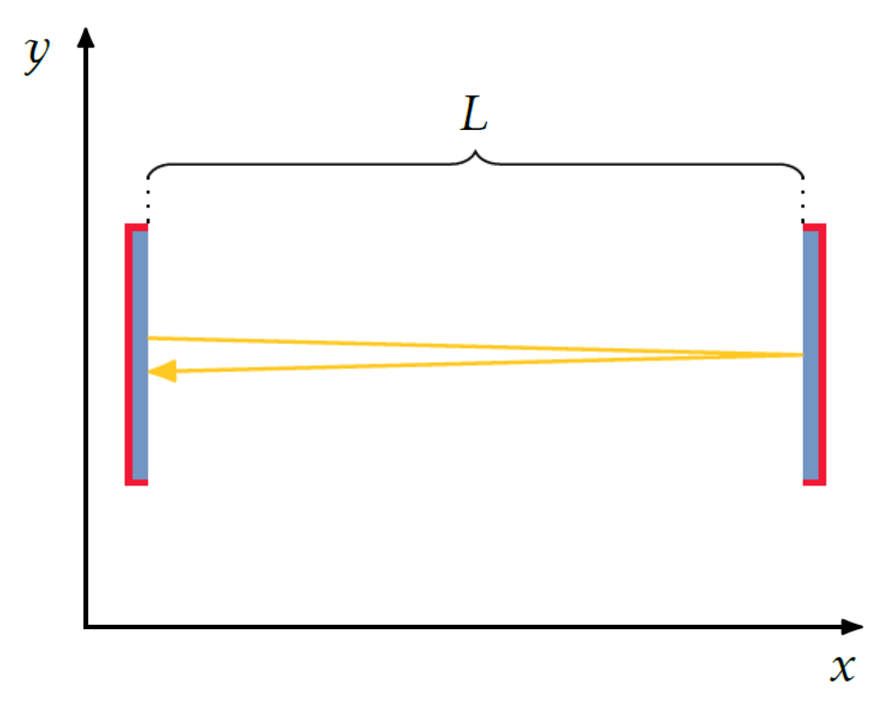
\includegraphics[width = .5\columnwidth]{Rel/RelLorent/lysur.eps}
    \caption{Det roterede lysur i sit hvilesystem. For observatører bevæger uret sig i $x$-retningen. Kilde: figur 2.1 \cite{uggerhojSpecielRelativitetsteori2016}.}
    \label{rel:fig:roteret_lysur}
\end{figure}

Vender vi tilbage til myonerne, vil afstanden, de skal tilbagelægge for at nå Jordens overflade, være langt mindre, idet verden trækkes sammen i bevægelsesretningen, for et objekt i bevægelse.
Man kan også observere længdeforkortning andre steder. Et eksempel er indenfor elektronkrystallografi, hvor man sender elektroner ind imod en krystal. Jo højere hastighed, man sender elektronerne ind med, desto mere komprimeret virker krystallen.
\subsubsection{Mangel på samtidighed}\label{rel:sec:samtidighed}

\subsubsection{Synkronisering af ure} \label{rel:sec:sync}

Vi kan forestille os, at vi ønsker at synkronisere to ure, så to forskellige personer kan være enige om tiden. Dette kan gøres ved at sende et lysglimt indeholdende information omkring afsendingstidspunktet fra ur A til ur B. Lige ved modtagelsen af lysglimtet afsendes et nyt lysglimt, indeholdende information omkring dettes afsendingstidspunkt, fra ur B til ur A. Når dette lysglimt når ur A sammenlignes afsendingstidspunktet for lysglimtet fra ur B med tidspunktet for afsendingen af det første lysglimt fra ur A og modtagelsen af lysglimtet fra ur B, se \cref{rel:fig:EinsteinSyncronization}a. Befinder afsendingstidspunktet for lysglimtet fra ur B sig midt mellem de to andre tidspunkter, da er urene synkroniserede. Eksempelvis afsender ur A kl. 12.00 et lysglimt til ur B, som modtager dette kl. 13.00, der straks sender et lysglimt tilbage til ur A, som modtager dette kl. 14.00. Kl. 13.00 ligger midt mellem kl. 12.00 og kl. 14.00, hvorfor de to ure er synkroniserede. Denne metode til synkronisering af ure kaldes for \emph{Einsteinsynkronisering}. Dette gør sig gældende for ure, der enten er stillestående eller i ens bevægelse, men ikke for ure i indbyrdes (relativ) bevægelse. Dette kan ses ved at benytte samme opstilling som før, blot hvor det ene ur er i bevægelse i forhold til det andet. Er ur B i bevægelse væk fra ur A, \cref{rel:fig:EinsteinSyncronization}b, da vil lysglimtet stadig tilbagelægge den samme vejlængde frem og tilbage, hvorfor samme konklusion som ovenfor fås, at urene \emph{er} synkroniserede. Er ur A derimod i bevægelse væk fra ur B, \cref{rel:fig:EinsteinSyncronization}c, da vil lysglimtet fra ur B til ur A have længere vej at tilbagelægge end lysglimtet fra ur A til ur B, hvorfor afsendingstidpunktet for lysglimtet fra ur B ikke vil ligge midt mellem afsendings- og modtagningstidspunkterne ved ur A. Ud fra proceduren kan der derved konkluderes, at de to ure \emph{ikke} er synkroniserede. Men ser man på det tilfældet, hvor ur B bevæger sig væk fra ur A, blot fra ur B's synspunkt, da ses ur B som værende stationært, mens ur A bevæger sig væk fra ur B, altså at de to tilfælde -- \cref{rel:fig:EinsteinSyncronization}b og \ref{rel:fig:EinsteinSyncronization}c -- er ens, blot set fra forskellige hvilesystemer. Ifølge relativitetsprincippet må synkroniseringen ikke afhænge af, om man ser situationen fra det ene eller det andet hvilesystem, hvorfor det må konkluderes, at to ure i indbyrdes bevægelse ikke kan synkroniseres.

\begin{figure}
    \centering
    \includegraphics[width=0.85\textwidth]{Rel/RelLorent/EinsteinSynkronisering.png}
    \caption{Einsteinsynkronisering. a) Ved at sende informationer om urenes
visning frem og tilbage, ved brug af lyssignaler, kan det afgøres om urene er synkroniserede. b) Forsøg på synkronisering mens ur B er i bevægelse væk fra ur A. c) Forsøg på synkronisering mens ur A er i bevægelse væk fra ur B. \newline Kilde: figur~3.1 og 3.2 i \cite{uggerhojSpecielRelativitetsteori2016}.}
    \label{rel:fig:EinsteinSyncronization}
\end{figure}

En anden måde at se, at synkronisering af ure i indbyrdes bevægelse ikke er mulig, er at huske tilbage til \cref{rel:sec:Tidsforlaengelse}, hvor vi så, at ``et ur i bevægelse går langsomt''. Selvom de to ure kunne synkroniseres, da ville overensstemmelsen gå tabt med det samme, da urene bevæger sig med forskellige hastigheder, hvilket resulterer i samme konklusion som ovenfor.


\subsubsection{Einsteins togeksperiment} \label{rel:sec:tog}

For at beskrive manglen på samtidighed lidt mere visuelt, gøres brug af et tankeeksperiment kaldet \emph{Einsteins togeksperiment}. Einsteins togeksperiment omhandler to personer, Fulbert og Beatrice, samt to ure. Fulbert er placeret på en togperron midt mellem de to stillestående ure, der er synkroniserede, mens Beatrice er placeret midt i toget, der kører forbi perronen. Afstanden mellem urene er præcis sådan, at idet Fulbert og Beatrice er lige ud for hinanden, da vil togets for- og bagende være præcist ud for hvert deres ur. På nøjagtig dette tidspunkt, f.eks. kl. 12.00, udsendes et lysglimt, en refleksion af lyset fra urskiven, da viserne viste nøjagtigt kl. 12.00, fra hvert af urene mod Fulbert og Beatrice. Fulbert modtager begge lysglimt samtidig og konkluderer da, at lysglimtene blev udsendt samtidig, altså at urene er synkroniserede. I løbet af den tid der går, fra lysglimtene bliver afsendt fra urene, og til lysglimtene krydser hinanden ved Fulbert, har toget med Beatrice bevæget sig fremad, se \cref{fig:EinsteinsTrainExperiment}. Lysglimtene mødes altså ikke i midten af toget, men tættere på bagenden af toget. Selvom Fulbert ser de to glimt som værende afsendt samtidig, da vil Beatrice konkludere, at lysglimtet fra uret ved togets forende er afsendt først, da dette lysglimt visende kl. 12.00 blev set først i toget, hvorefter lysglimtet fra det andet ur, også visende kl. 12.00, blev set, og Beatrice var placeret midt mellem de to ure, da lysglimtet blev udsendt.
%
\begin{figure}[t]
    \centering
    \begin{subfigure}[t]{.31\textwidth}
        \centering
        \includegraphics[width=\columnwidth]{Rel/RelLorent/EinsteinTrainExperiment1.PNG}
        \caption{Fulbert er placeret midt på en togperron, og Beatrice er placeret midt i et forbikørende tog.}
        \label{fig:EinsteinsTrainExperiment1}
    \end{subfigure}
    %
    \hfill
    %
    \begin{subfigure}[t]{.31\textwidth}
        \centering
        \includegraphics[width=\columnwidth]{Rel/RelLorent/EinsteinTrainExperiment2.PNG}
        \caption{Fra Fulberts perspektiv udsendes lysglimtene samtidig i togets for- og bagende (punkt A og B).}
        \label{fig:EinsteinsTrainExperiment2}
    \end{subfigure}
    %
    \hfill
    %
    \begin{subfigure}[t]{.31\textwidth}
        \centering
        \includegraphics[width=\columnwidth]{Rel/RelLorent/EinsteinTrainExperiment3.PNG}
        \caption{Idet Beatrice (og dermed toget) bevæger sig mod punkt A, vil hun opleve, at lysglimetet, der blev udsendt fra togets forende, blev udsendt før det i togets bagende, idet lyset bevæger sig med samme hastighed fra de to lysglimt.}
        \label{fig:EinsteinsTrainExperiment3}
    \end{subfigure}
    \caption{Einsteins togeksperiment. Kilde: \cite{uggerhojSpecielRelativitetsteori2016}.}
    \label{fig:EinsteinsTrainExperiment}
\end{figure}
%
Da Beatrice modtager signalet fra ur A, før hun modtager signalet fra ur B,
% Set fra Beatrices perspektiv viser ur A -- det for hende bagerste perronur, da Beatrice ser perronen med Fulbert og urene bevæge sig den modsatte retning af, hvad Fulbert ser toget bevæge sig -- kl. 12.00 og først lidt senere viser ur B -- det for hende forreste perronur -- kl. 12.00. Beatrice 
konkluderer hun, at ur A er tidsmæssigt foran, hvorimod Fulbert konstaterede at de var synkroniserede.

Konklusionen er, at begivenheder, der sker samtidigt for Fulbert, ikke nødvendigvis gør det for Beatrice. Dette kan opsummeres som:
%
\begin{quote}
	Begivenheder, der sker på samme \emph{tid}, men på forskellige \emph{steder} for én observatør, sker til forskellige \emph{tider} for en observatør, der er i bevægelse i forhold til den første.
\end{quote}
%
I relativitetsteori behandles tid og rum på lige fod, og benyttes nu denne lighed kan ovenstående sætning direkte omskrives til:
%
\begin{quote}
	Begivenheder der sker på samme \emph{sted}, men til forskellige \emph{tider} for én observatør, sker på forskellige \emph{steder} for en observatør, der er i bevægelse i forhold til den første.
\end{quote}
%
Dette beskriver netop manglen på absolut samtidighed.
\subsubsection{Lysets hastighed som en ultimativ hastighed}

Kigger man på den klassiske, ikke-relativistiske mekanik, der er beskrevet af Newtons love, kan en partikel beskrives ved blandt andet dens kinetiske energi, $K$ (også kendt som $E_{\textup{kin}}$), som afhænger af partiklens fart, $v$:
%
\begin{align} \label{rel:eq:KineticEnergy}
    K = \frac{1}{2}m_0v^2.
\end{align}
%
Her er $m_0$ hvilemassen, hvilket er massen af partiklen i det system, hvor partiklen er i hvile, altså i hvilesystemet. Det viser sig nemlig, at det ikke er den samme masse, som hvis partiklen var i bevægelse.

\begin{figure}[t]
    \centering
    \includegraphics[width=0.5\textwidth]{Rel/RelLorent/EksperimentalSetupElectronVelocity.pdf}
    \caption{En ladet partikel accelereres gennem et spændingsfald $V$ og fortsætter udenfor spændingsfaldet upåvirket (og dermed med konstant hastighed). Partiklens flyvetid mellem to steder A og B måles, og fra dette udregnes partiklens hastighed.}
    \label{fig:ExperimentElectronVelocity}
\end{figure}

Vi ønsker nu at bekræfte udtrykket i \cref{rel:eq:KineticEnergy}, hvorfor vi opstiller et eksperiment, som kan måle hastigheden af en partikel som funktion af dens kinetiske energi. Et sådan eksperiment er skitseret på \cref{fig:ExperimentElectronVelocity}. Her accellereres en elektrisk ladet partikel fra hvile gennem et spændingsfald $V$, således at den opnår den kinetiske energi $K = qV$, hvor $q$ er partiklens ladning. Udenfor spændingsfaldet fortsætter partiklen upåvirket af kræfter, hvorfor den opretholder en konstant fart, $v$. Farten findes ud fra bestemmelse af flyvetiden mellem to punkter, f.eks. $A$ og $B$, hvorimellem længden, $L$, er kendt:
%
\begin{align}
    v &= \frac{L}{t_\textup{B} - t_\textup{A}},
    %
    \intertext{hvor $t_\textup{A}$ og $t_\textup{B}$ er tiden ved punkt $A$ og $B$ respektivt. Måler man nu hastigheden af elektroner på denne måde, og sammenlignes med det klassiske udtryk fra \cref{rel:eq:KineticEnergy}, hvor hastigheden er isoleret (her i enheder af lysets hastighed),}
    %
    \frac{v}{c} &= \sqrt{\frac{2K}{m_0c^2}}, \label{rel:eq:ExpectedExpressionForVelocity}
\end{align}
%
fås \cref{rel:fig:ClassicalVsRelativisticVelocity}.De røde punkter er målepunkter, mens den stiplede sorte kurve angiver det forventede udtryk for $v$ fra \cref{rel:eq:ExpectedExpressionForVelocity}. Overensstemmelsen mellem det forventede udtryk og de målte data er ikke specielt god. I stedet for en liggende parabel, stammende fra kvadratroden i \cref{rel:eq:ExpectedExpressionForVelocity}, flader grafen ud og går øjensynligt mod en grænseværdi på $v/c = 1$, altså $v = c$. Uanset det valgte spændingsfald, så er det altså ikke muligt at drive partiklens hastighed over lysets hastighed, hvilket er et uventet resultat, hvis man følger den Newtonske mekanik. Det kan vises, at det korrekte relativistiske udtryk for en partikels hastighed som funktion af dens kinetiske energi er
%
\footnotetext{At en funktion nærmer sig en grænseværdi asymptotisk, betyder at funktionen kommer uendeligt tæt på, men aldrig rammer helt præcist. Et eksempel på en sådan funktion er $f(x) = e^{-x} = 1/e^x$. Når $x$ går mod uendeligt, er $f(x)$ lig med 1 divideret med noget uendelig stort, hvorfor $f(x)$ må være uendelig lille. $f(x)$ kan aldrig blive præcist lig med nul, men den kan komme uendeligt tæt på, hvorfor man siger at $f(x)$ går asymptotisk mod $0$ for $x \rightarrow \infty$.\label{asymptot}}
%
\begin{align} \label{rel:eq:ExpressionForVelocity}
    v = c \cdot \sqrt{1 - \dfrac{1}{\left(K/m_0c^2 + 1\right)^2}}.
\end{align}
%
Uoverensstemmelsen mellem det klassiske udtryk og de målte værdier på \cref{rel:fig:ClassicalVsRelativisticVelocity} vokser med den kinetiske energi, idet de målte værdier asymptotisk\footref{asymptot} går mod grænseværdien
%
\begin{align} \label{rel:eq:LimitValueForVelocity}
    v_l &\simeq \SI{3.0e8}{\frac{\metre}{\second}}.
\end{align}
%
Denne hastighed overstiger langt de almindelige dagligdagshastigheder, og for små hastigheder, $v \ll c$, er forskellen mellem de målte og klassisk forventede hastigheder forsvindende lille, hvorfor den Newtonske mekanik er god i disse situationer\footnote{Hvis man har lyst til en udfording, kan man bruge teorien om Taylorrækker til at vise, at \cref{rel:eq:ExpressionForVelocity} kan approksimeres med \cref{rel:eq:ExpectedExpressionForVelocity} i grænsen hvor $K/m_0c^2$ er et lille.}. Den klassiske, ikke-relativistiske mekanik bryder altså ikke sammen, men man skal blot overveje, hvornår man opnår så store hastigheder, at de er i det relativistiske område.
%
\begin{figure}[t]
    \centering
    \includegraphics[width=0.7\textwidth]{Rel/RelLorent/ClassicalVsRelativisticVelocityUggerhoej.PNG}
    \caption[]{Hastigheden af elektroner i enheder af lysets hastighed, som funktion af den kinetiske energi i enheder af hvilemasse for en elektron. Den sorte stiplede kurve angiver det klassiske, ikke relativistiske udtryk, de røde punkter er eksperimentelle målepunkter, og den stiplede grønne linje angiver lysets hastighed. Det ses, at de målte værdier asymptotisk\footref{asymptot}~nærmer sig grænseværdien $v = c$, altså kommer $v$ tættere og tættere på $c$ jo større den kinetiske energi bliver. Kilde: figur 5.1 i \cite{uggerhojSpecielRelativitetsteori2016}.}
    \label{rel:fig:ClassicalVsRelativisticVelocity}
\end{figure}

Vi bemærker, at vi kun kender til ét fænomen i naturen, hvis hastighed er lige så stor som $v_l$ fra \cref{rel:eq:LimitValueForVelocity}, hvilket er lysets udbredelse i vakuum:
%
\begin{align}
    c &= \SI{299792458}{\frac{\metre}{\second}},
\end{align}
%
hvilket, indenfor den eksperimentelle usikkerhed af de målinger, der giver grænseværdien, er det samme som grænseværdien.
Det kan konkluderes, at eftersom elektronen er en af de letteste bestanddele af almindeligt stof, med en hvilemasse forskellig fra nul, ikke kan bringes op til lysets hastighed, så må man forvente, at \emph{intet} med en hvilemasse forskellig fra $0$, kan bringes op til denne hastighed.
\section{Lorentztransformationerne}
Vi har snakket en del om forskellige observatører, men hvad menes der egentligt med en observatør.
Den specielle relativitetsteori beskriver inertialsystemer, så alle observatører vil være i et inertialsystem.
En observatør i inertialsystemet $S$ vil således se positionerne $x$ og tiden $t$.
En observatør i inertialsystemet $S'$ vil derimod se positionerne $x'$ og tiden $t'$.
Når man har et inertialsystem vil andre inertialsystemer være i bevægelse med konstant hastighed i forhold til hinanden.
Så inertialsystemet $S'$ bevæger sig med hastigheden $v$ i forhold til inertialsystemet $S$.
Vi leder efter en måde at oversætte imellem forskellige inertialsystemer, en såkaldt transformation.
I den klassiske mekanik, hvor tiden er absolut, bruges Galileitransformationerne, ligning \eqref{SR:GalileiTransformationen}, %er det blot et spørgsmål om at korregere for inertialsystemernes bevægelse
\begin{subequations}
\label{eq:galilei}
\begin{align}
    x'&=x-vt \: ,\\
    t'&=t \: ,
\end{align}
\end{subequations}
% hvilket kaldes Galileitransformationen.
Vi har dog vist at tid ikke er absolut, hvis man kræver at lysets hastighed er det.
Vi bliver derfor nød til at finde et andet sæt transformationer; Lorentztransformationerne.


\subsection{Krav til Lorentztransformationerne} \label{sec:krav}
Før vi vil udlede den specifikke form af Lorentztransformationerne, vil vi først kigge på nogle krav, som transformationerne skal opfylde.
Helt generelt søger vi to funktioner for $x'$ og $t'$ med $x$, $t$ og $v$ som variable:
\begin{subequations}
\begin{align}
    x'&=\xi(v,x,t) \: ,\\
    t'&=\Xi(v,x,t) \: ,
\end{align}
hvor $\xi$ og $\Xi$ er henholdsvis den lille og den store version af det græske bogstav \textit{ksi}, som er vilkårlige navne for de to transformationer.
\end{subequations}
\begin{enumerate}
    \item Vi er kun interesserede i transformationer imellem inertialsystemer. Det betyder, at et legeme, der bevæger sig med konstant hastighed i $S$, også gør det i $S'$.
    Det viser sig, at det betyder, at transformationerne kun kan afhænge af $x$ og $t$ i første (ingen begrænsninger på $v$ afhængigheden her).
    Man siger da, at tranformationen er lineær i $x$ og $t$.
    Lad os se på et modeksempel, for at demonstrere hvad der sker, hvis transformationerne ikke er lineær.
    Vi ser på transformationerne
    \begin{align*}
        x'&=d(v)x^2+f(v)t^2 \: ,\\
        t'&=g(v)x+h(v)t \: ,
    \end{align*}
    hvor $d(v)$, $f(v)$, $g(v)$ og $h(v)$ er arbitrære funktioner af $v$. Lad os se på en partikel der bevæger sig med jævn hastighed $u$ i $S$, dvs.
    \begin{equation*}
        x=ut \: .
    \end{equation*}
    Så giver vores ikke-lineære transformation
    \begin{align*}
        x' &= d(v)u^2t^2+f(v)t^2 = \left(d(v)u^2+f(v)\right)t^2 \: ,\\
        t' &= g(v)ut+h(v)t = \Big(g(v)u+h(v)\Big)t \: .
    \end{align*}
    Her kan $t$ elimineres, hvilket efterlader $x'$ som en funktion af $t'$
    $$
        x'=\frac{d(v)u^2+f(v)}{\big(g(v)u+h(v)\big)^2}(t')^2\propto (t')^2 \: .
    $$
    Tegnet $\propto$ betyder proportionalt med og det vigtige er at $x'$ er en konstant ganget med $(t')^2$, hvilket betyder hastigheden ikke er jævn -- det er nu accelerationen som er konstant.
    % I $S'$ bevæger partikelen ikke med jævn hastighed, så 
    Denne transformation skifter derfor ikke imellem inertialsytemer.
    Det kan derfor konkluderes at transformationerne må være på formen
    \begin{subequations}
    \begin{align}
        x' &= d(v)x+f(v)t \: , \\
        t' &= g(v)x+h(v)t \: ,
    \end{align}
    hvor $d(v)$, $f(v)$, $g(v)$ og $h(v)$ igen er arbitrære funktioner af $v$.
    \end{subequations}
    \item transformationerne skal være symmetriske.
    Siden både $S$ og $S'$ er inertialsystemer, må vi også kunne transformere den anden vej, altså finde $x$ og $t$, som funktion af $x'$ og $t'$.
    Ikke nok med det, når $S'$ bevæger sig med farten $v$ i forhold til $S$, så må $S$ bevæge sig med samme fart i den modsatte retning set fra $S'$.
    Så den omvendte\footnote{Mere præcist kalder man den omvendte transformation for den \textit{inverse transformation}. To transformationer, $T$ og $T'$ kaldes hinandens inverse transformationer hvis $TT' = T'T = 1$. På samme måde er $1/2$  og $2$ hinandens inverse da $1/2\cdot 2 = 2\cdot 1/2 = 1$.} transformation må være
    \begin{subequations}
    \begin{align}
        x&=d(-v)x'+f(-v)t' \:  ,\\
        t&=g(-v)x'+h(-v)t' \: .
    \end{align}
    \end{subequations}
    \item For små hastigheder skal Lorentztransformationerne nærme sig Galileitransformationerne. Dette er korrespondanceprincippet\footnote{Har man en fysisk teori, der virker til at beskrive nogle bestemte fænomener, så skal en ny teori forudsige det samme som den gamle på det område, hvor den gamle virker. Vi kan se at Newtonsk mekanik ikke virker for store hastigheder, men for små hastigheder virker den helt fint. Derfor må relativitetsteorien give samme resultater for små hastigheder som Newtonsk mekanik, da disse resultater passer med eksperimenter.} i aktion.
    Vi ved, at Galileitransformationerne virker ved lave hastigheder, så hvis Lorentztransformationerne forudsiger noget andet dér, må det være Lorentztransformationerne, der er noget galt med.
    \item Noget, der bevæger sig med lysets hastighed i ét inertialsystem, vil gøre det i alle inertialsystemer.
    Dette krav garanterer, at lysets hastighed er den samme for alle observatører.
    Siden vi har udledt tidsforlængelse og længdeforkortning ud fra postulatet om at lysets hastighed er absolut, kan vi bruge dem, når vi udleder Lorentztransformationerne.
\end{enumerate}
Det er værd at nævne at Galileitransformationerne allerede opfylder de tre første krav, og det er det sidste der fører os til Lorentztransformationerne.


\subsection{Udledning af Lorentztransformationerne}
Ud fra kravene i afsnit \ref{sec:krav} kan Lorentztransformationerne udledes. Det er vigtigt at vide hvilke fysiske krav man sætter til koordinattransformationerne, men det er simplere at udnytte den viden vi har om længdeforkortelse fra afsnit \ref{sec:Laengdeforkortelse}. Lad os se på afstanden fra origo ud til $x'$ i $S'$.
Dette svarer til længden af en stang i hvile i $S'$, så vi kan skrive
\begin{equation}
    x'=L'=L_0 \: .
\end{equation}
$L_0$ er her stangens længde i sit eget hvilesystem og $L'$ er længden af stangen i $S'$. I dette tilfælde er $S'$ stangens inertialsystem, hvorfor $L_0 = L'$.
I $S$ bevæger stangen sig med en fart $v$ og yderligere er den længdeforkortet, så
\begin{equation}
    x=vt+\frac{L_0}{\gamma} = vt+\frac{x'}{\gamma} \: .
\end{equation}
Nu kan vi isolere $x'$, der er
\begin{equation}
    x'=\gamma(x-vt) \: . \label{lorentzx}
\end{equation}
Man kan gøre præcis det samme med en stang i hvile i $S$, hvilket giver
\begin{equation}
    x=\gamma(x'+vt') \: .\label{lorentzxinv}
\end{equation}
Sætter vi $x'$ fra ligning \eqref{lorentzx} ind i ligning \eqref{lorentzxinv}, så får vi at
\begin{equation}
    x=\gamma\Big(\gamma(x-vt)+vt'\Big) = \gamma^2(x-vt) + \gamma vt' \: ,
\end{equation}
hvilket også kan skrives som
\begin{equation}
    \gamma vt' = x - \gamma^2(x-vt) \: .
\end{equation}
hvori vi kan isolere $t'$:
\begin{equation}
    t' = \frac{1}{\gamma v}\Big[x - \gamma^2(x-vt)\Big] = \frac{1}{v}\left(\frac{x}{\gamma}-\gamma x\right) + t = \gamma \left(\frac{x}{v}\left(\frac{1}{\gamma^2}-1\right)+t\right)=\gamma\left(t-\frac{vx}{c^2}\right) \: .
\end{equation}
Igen kan man gøre det samme for $t'$, hvilket giver
\begin{equation}
    t=\gamma\left(t'+\frac{vx'}{c^2}\right) \: ,
\end{equation}
så Lorentztransformationerne er
\begin{subequations}
\begin{align}
    x'&=\gamma x-\gamma vt \: , \label{rel:LorentzXComposant} \\
    t'&=\gamma t-\gamma\frac{vx}{c^2} \: . \label{rel:LorentzTComposant}
\end{align}
\end{subequations}
Omskrives transformationerne en lille smule er det muligt at tydeliggøre sammenhængen mellem tid og rum, som findes i den specielle relativitetsteori.
Det gøres ved at gange tiden med $c$, således at denne transformation også angives i enheder af længde.
Det giver transformationerne
\begin{subequations}
\begin{align}
    x'&=\gamma x-\gamma\beta ct \: , \label{rel:LorentzXComposantWithBeta}\\
    ct'&=\gamma ct-\gamma\beta x \: , \label{rel:LorentzTComposantWithBeta}
\end{align}
\end{subequations}
hvor vi har benyttet beta-faktoren $\beta = v/c$ for at gøre transformationerne pænere. \\

Et smart trick ved Lorentztransformationerne er, at hvis man har transformationen af en variabel fra $S$ til $S'$, så fås transformationen fra $S'$ til $S$ ved at sætte mærker på de umærkede koordinater og fjerne mærkerne fra de tidligere mærkede koordinater, samt skifte fortegn på alle $v$'erne. Bemærk at $\gamma$ ikke skifter fortegn, da hastigheden optræder i anden. Vi kan tjekke at det passer på ligning \eqref{lorentzx}. For at få de omvendte transformationer skal $x \rightarrow x'$, $x' \rightarrow x$, $t \rightarrow t'$, $t' \rightarrow t$ og der skal skiftes fortegn på $v$:
%
% \begin{figure}[H!]
% \centering
\begin{center}
\begin{tikzpicture}
\matrix (m) [matrix of math nodes,
             row sep=3mm]
{
    x' & = & \gamma & (x & - & vt)    \\
    x  & = & \gamma & (x' & + & vt')    \\
};
\draw[thick, ->] (m-1-1) -- (m-2-1);
\draw[thick, ->] (m-1-4) -- (m-2-4);
\draw[thick, ->] (m-1-5) -- (m-2-5);
\draw[thick, ->] (m-1-6) -- (m-2-6);
\end{tikzpicture}
\end{center}
% \end{figure}

\section{Rumtidsintervallet}
I den specielle relativitetsteori er hverken tid eller rum det samme for forskellige observatører.
Vi har derfor brug for en anden måde at relatere to begivenheder, som alle observatører kan blive enige om.
Vi har brug for en størrelse, der antager samme værdi i alle inertialsystemer -- en såkaldt {\em invariant} størrelse.

Lad os se på to begivenheder, en der sker i $x_1$ til tiden $t_1$ og en anden der sker i $x_2$ til tiden $t_2$ i inertialsystemet $S$.
Vi ønsker nu at se på hvad der sker med de to begivenheder hvis vi skifter til inertialsystemet $S'$. I $S$ er afstanden og tidsforskellen imellem de to begivenheder givet ved:
\begin{subequations}
\begin{align}
    \Delta x&=x_2-x_1 \: , \\
    \Delta t&=t_2-t_1 \: .
\end{align}
\end{subequations}
For at finde afstanden og tidsforskellen i $S'$ benytter vi Lorentztransformationerne.
\begin{subequations}
\begin{gather}
    \Delta x' = x'_2-x'_1=\gamma x_2-\gamma vt_2-\gamma x_1+\gamma v t_1=\gamma \Big(\Delta x- v\Delta t\Big) \: , \\
    \Delta t' = t'_2-t'_1=\gamma t_2-\gamma \frac{vx_2}{c^2}-\gamma t_1+\gamma \frac{vx_1}{c^2} = \frac{\gamma}{c} \left(c\Delta t - \frac{v\Delta x}{c} \right) \: .
\end{gather}
\end{subequations}
Nu lader vi os inspirere af, at når vi normalt måler afstande, bruger vi $\Delta x^2$ led\footnote{I tre dimensioner er afstanden imellem to punkter $\Delta l=\sqrt{\Delta x^2+\Delta y^2+\Delta z^2}$.}.
Det giver
\begin{subequations}
\begin{gather}
    \Delta x'^2=\gamma^2\Big(\Delta x^2+v^2\Delta t^2-2v\Delta x\Delta t\Big) \label{sr:delta_x'}\\
    \Delta t'^2 = \frac{\gamma^2}{c^2} \left(c^2\Delta t^2+\frac{v^2\Delta x^2}{c^2}-2v\Delta x\Delta t\right) \label{sr:delta_t'}
\end{gather}
\end{subequations}
Det er nu smart at trække ligning \eqref{sr:delta_t'} fra ligning \eqref{sr:delta_x'} efter at have flyttet $c^2$ over på den anden side, så enhederne er ens i begge ligninger. Vi bemærker også at de to sidste led i begge parenteser er ens, %så vi lader dem gå ud med hinanden,
hvorved vi får
\begin{equation}
\Delta x'^2-c^2\Delta t'^2=\gamma^2\left(\Delta x^2+v^2\Delta t^2-c^2\Delta t^2-\frac{v^2}{c^2}\Delta x^2\right) \: .
\end{equation}
Flytter vi en anelse rundt på ledene i parentesen får vi, at
\begin{equation}
    \Delta x'^2-c^2\Delta t'^2=\gamma^2\left(1-\frac{v^2}{c^2}\right)(\Delta x^2-c^2\Delta t^2)=\Delta x^2-c^2\Delta t^2 \: .
\end{equation}
Vi ser nu, at denne størrelse er ens for de to observatører -- den ændrer sig ikke under en Lorentztransformation.
Det er faktisk ligegyldigt hvilket inertialsystem størrelsen $\Delta x^2-c^2\Delta t$ regnes i -- den er den samme i alle inertialsystemer.
Vi har netop fundet en invariant størrelse og kalder denne størrelse rumtidsintervallet. Den skrives som
\begin{equation}
\Delta s^2=\Delta x^2-c^2\Delta t^2 \: .
\end{equation}
Det smarte ved en invariant størrelse er netop det, at den ikke ændrer sig, når vi skifter inertialsystem. Således er invariante størrelser noget, som alle observatører, \emph{uanset deres inertialsystem}, er enige om.  

Det betyder, at vi kan vælge netop det system, der gør det så let som muligt at analysere en fysisk situation, hvilket ofte er en partikels hvilesystem, da dens hastighed her per definition er $0$. 




\begin{subequations}
\begin{align}
    \left(x^0\right)' &= \gamma \cdot \left(x^0 - \frac{v \cdot  x^1}{c}\right) \label{rel:eq:lorx0} \\
    \left(x^1\right)' &= \gamma \cdot \left(x^1 - \frac{v\cdot x^0}{c}\right) \label{rel:eq:lorx1}\\
    \left(x^2\right)' &= x^2 \\
    \left(x^3\right)' &= x^3 
\end{align}
\label{rel:eq:lorentrans}
\end{subequations}

\section{Rumtidsdiagrammer} %Anna tager den lol
%
\begin{figure}[]
    \centering
    \includegraphics[trim = 100 110 100 80, clip, width = .8\textwidth]{Rel/Billeder/EmptyDiagram.pdf}
    \caption{Et simpelt rumtidsdiagram. Du er måske vandt til at se position som en funktion af tid (såkaldte ``$x(t)$-diagrammer''), men her er det altså omvendt.}
    \label{rel:fig:rumtid_empt}
\end{figure}
%
Nu har vi brugt rigeligt tid på adskillige regnetekniske udfordringer indenfor speciel relativitetsteori, så lad os lige stoppe op, og gøre hvad fysikere gør bedst, når det kommer til komplicerede problemer: tegne.
Indenfor speciel relativitetsteori hedder det visuelle metode, man ofte anvender, \emph{rumtidsdiagrammer} (eller \emph{Minkowski diagrammer} efter deres opfinder, Hermann Minkowski). I et rumtidsdiagram sætter man $x^0$ koordinatet, altså tiden, op af den lodrette akse, og $x^1$-koordinatet ud af den vandrette akse. Et eksempel på et rumtidsdiagram kan ses i \cref{rel:fig:rumtid_empt}.

Vi kalder det et rumtidsdiagram, fordi man i relativitetsteori sætter koordinater, der beskriver tid, og koordinater, der beskriver sted, på samme fod. Dette er også hvorfor at lysets hastighed dukker op i \cref{rel:eq:four}, for hvis man ganger en tid med en hastighed, får man en længde\footnote{Nogen gange bliver fysikere endda så sløve at de ikke engang gider at skrive $c$ når det ellers burde være der, men i dette kompendium skriver vi det ud.}:
%
\begin{align} \label{rel:eq:xo_enhed}
    \big[ x^0 \big] = \big[ ct \big] = \frac{\si{\meter}}{\SI{}{\second}} \cdot \si{\second} = \si{\meter}.
\end{align}
%
I \cref{rel:eq:xo_enhed} betyder notationen med de firkantede parenteser enheden af, hvad der står i dem. Eksempelvis betyder $[ct]$ ``enheden for $ct$''. På den måde kan man altså måle tid i meter (eller længder i sekunder). Vi snakker altså ikke kun om rum og tid som seperate ting, men som en samlet \emph{rumtid}.

Vi bruger rumtidsdiagrammer til at vise objekters bevægelse igennem rumtid, for eksempel kan man have en bold der ligger stille på gulvet. Det er måske ikke den mest spændende scenarie, at forestille sig, men husk på at nok ligger bolden stille i rummet, men den bevæger sig altid fremad i tid! Derfor ville vi tegne den i et rumtidsdiagram som en linje, der holder samme værdi på $x^1$-aksen, men fortsætter op af $x^0$-aksen; med andre ord, en lodret streg. Stregen som et objekt danner på et rumtidsdiagram kalder vi for objektets \emph{verdenslinje}. Hvis vi nu lader bolden trille med den konstante hastighed $v$ i retningen af $x^1$-aksen, vil dens position i rummet selvfølgelig også ændre sig; altså vil dens verdenslinje være en ret linje. Rumtidsdiagrammerne for disse bolde kan findes i \cref{rel:fig:ball}.

\begin{figure}
    \centering
    \includegraphics[trim = 0 100 0 0, clip, width = \textwidth]{Rel/Billeder/Ball_diagram.pdf}
    \caption{(a) Rumtidsdiagram med verdenslinje for en bold der ligger stille. Læg mærke til, at boldens $x^1$-værdi altid er den samme, men den bevæger sig fremad (eller opad) i tid, $x^0$. (b) Rumtidsdiagram for en bold, der triller med konstant hastighed. Læg mærke til, at bolden her både ændrer sin $x^1$-værdi og sin-$x^0$ værdi -- den bevæger både sig i rum og tid.}
    \label{rel:fig:ball}
\end{figure}

\subsection{Lorentz transformationer i rumtidsdiagrammer}

Relativitetsteori handler i sin essens om, hvordan ting ser ud i forskellige referencesystemer. Derfor er det også vigtigt, at få en intuitiv forståelse af hvordan transformationerne imellem referencesystemer ``ser ud''. Tilbage i \cref{rel:sec:trans} udledte vi formlen for Lorentztransformation, \cref{rel:eq:lorentrans}, som er grundstenen bag speciel relativitetsteori. Lad os prøve at se hvordan sådan en transformation ser ud, hvis vi tegner den ind i et rumtidsdiagram. Kigger tilbage på \cref{rel:eq:lorx0,rel:eq:lorx1},
%
\begin{subequations}
\begin{align}
    \left(x^0\right)' &= \gamma \cdot \left(x^0 - \frac{v \cdot  x^1}{c}\right), \label{rel:eq:lorentz_rumtid_tid} \\
    \left(x^1\right)' &= \gamma \cdot \left(x^1 - \frac{v\cdot x^0}{c}\right), \label{rel:eq:lorentz_rumtid_sted}
\end{align}
\end{subequations}
%
så lad os overveje, hvad disse ligninger visuelt betyder for rumtidsdiagrammet. Ligningerne transformerer koordinater fra ét inertialsystem $S$, til et andet system $S'$, som bevæger sig med konstant hastighed $v$ i $x^1$-aksens retning relativt til $S$. $\left(x^0\right)'$ er tidskoordinatet i vores nye inertialsystem, $S'$, så hvis vi sætter $\left(x^0\right)' = 0$, får vi den vandrette akse i $S'$, altså $\left(x^1\right)'$-aksen. Ligeledes, hvis vi sætter $\left(x^1\right)' = 0$, finder vi den lodrette akse i $S'$. Lad os prøve at gøre dette, og repræsentere akserne i $S'$, i forhold til akserne i $S$. Dette gør vi først med $\left(x^0\right)' = 0$. Isoleres $x^0$ i \cref{rel:eq:lorentz_rumtid_tid} fås
%
\begin{align}
\begin{aligned}
    \left(x^0\right)' = 0 &= \gamma\cdot \left(x^0 - \frac{v\cdot x^1}{c}\right) = \gamma \cdot x^0 - \gamma \cdot \frac{v\cdot x^1}{c}  \\
    \implies -\gamma \cdot x^0 &= - \gamma \cdot \frac{v\cdot x^1}{c} = \gamma \cdot \frac{v\cdot x^1}{c} \\
    \implies x^0 &= \frac{v\cdot x^1}{c}
\end{aligned}
\end{align}
%
Dette svarer til en ret linje, som går igennem origo med hældningen $v/c$. Ligeså kan man sætte $\left(x^1\right)' = 0$ og finde den rette linje%
%
\begin{align}
    \left(x^0\right)'& = \frac{c\cdot x^1}{v}.
    %
    \intertext{Disse to rette linjer kan ses indtegnet i rumtidsdiagrammet for $S$ i \cref{rel:fig:TransDia}.
    Det ses, at akserne for $S'$ bliver ``trykket sammen'' i forhold til dem for $S$ -- jo størrere relativ hastighed, $v$, imellem de to inertialsystemer, desto mere bliver $S'$ trykket sammen. Man kunne eksempelvis kigge på vinklen imellem $x^1$-aksen og $\left(x^1\right)'$-aksen. Denne vinkel er den samme, som den imellem $x^0$-aksen og $\left(x^0\right)'$-aksen. Prøv om du kan tænke dig frem til hvorfor. Denne vinkel kan vi kalde for $\alpha$, og med en smule trigonometrisk snilde kan det vises, at}
    %
    \alpha &= \tan^{-1} \left(\frac{v}{c}\right).
\end{align}
%
Med dette resultat kan vi sågar sige, at jo større hastighed $v$, desto større bliver vinklen\footnote{Dette skyldes at $\tan^{-1}$ er hvad man kalder en \emph{monoton, strengt voksende} funktion -- altså at en større $x$-værdi medfører en større værdi af $\tan^{-1}(x)$.} $\alpha$. Denne vinkel kaldes \emph{boostvinklen}, da en Lorentztransformation også ofte kaldes et Lorentzboost.
% den viser hvor meget $S'$ er ``boosted'' relativt til $S$.
%
\begin{figure}[]
    \centering
    \includegraphics[trim = 100 150 200 0, clip, width =  0.49\textwidth]{Rel/Billeder/LorentzTransform.pdf}
    \includegraphics[trim = 100 150 200 0, clip, width = 0.49\textwidth]{Rel/Billeder/BoostAngle.pdf}
    \caption{Rumtidsdiagrammet for $S$, hvor akserne for $S'$ er indtegnet. Læg mærke til, at det ligner, at det nye inertialsystem bliver ``trykket sammen''. I (a) ses forskriften for de rette linjer, der udgør akserne i $S'$. I (b) ses boost-vinklen, $\alpha$, imellem akserne i $S$ og $S'$.}
    \label{rel:fig:TransDia}
\end{figure}



\section{Rumtidsinterval}






% ====================


I den specielle relativitetsteori er hverken tid eller rum det samme for forskellige observatører.
Vi har derfor brug for en ny måde at relatere to begivenheder, som alle observatører kan blive enige om.
Vi har brug for en størrelse, der antager samme værdi i alle inertialsystemer -- en såkaldt \emph{invariant} størrelse.

Lad os se på to begivenheder, en der sker i $x_1$ til tiden $t_1$, og en anden der sker i $x_2$ til tiden $t_2$ i inertialsystemet\footnote{Bemærk at det her er praktisk, at rumtidsindekset stod øverst, fordi vi så kan bruge et indeks nederst til at navngive en bestemt begivenhed, uden at blande de to sammen.} $S$.
Vi ønsker nu at se på, hvad der sker med de to begivenheder, hvis vi skifter til inertialsystemet $S'$. I $S$ er afstanden og tidsforskellen imellem de to begivenheder givet ved:
%
\begin{subequations}
\begin{align}
    \Delta x&=x_2-x_1, \\
    \Delta t&=t_2-t_1.
\end{align}
\end{subequations}
%
For at finde afstanden og tidsforskellen i $S'$ benytter vi Lorentztransformationerne:
%
\begin{subequations}
\begin{align}
    \Delta x' &= x'_2-x'_1=\gamma x_2-\gamma vt_2-\gamma x_1+\gamma v t_1=\gamma \Big(\Delta x- v\Delta t\Big), \\
    \Delta t' &= t'_2-t'_1=\gamma t_2-\gamma \frac{vx_2}{c^2}-\gamma t_1+\gamma \frac{vx_1}{c^2} = \frac{\gamma}{c} \left(c\Delta t - \frac{v\Delta x}{c} \right).
\end{align}
\end{subequations}
%
Nu lader vi os inspirere af, at når vi normalt måler afstande, bruger vi $\Delta x^2$-led\footnote{I tre dimensioner er afstanden imellem to punkter $\Delta l=\sqrt{\Delta x^2+\Delta y^2+\Delta z^2}$.}.
Det giver
%
\begin{subequations}
\begin{align}
    \left(\Delta x'\right)^2 &= \gamma^2\Big(\Delta x^2+v^2\Delta t^2-2v\Delta x\Delta t\Big) \label{rel:eq:delta_x'} \\
    \left(\Delta t'\right)^2 &= \frac{\gamma^2}{c^2} \left(c^2\Delta t^2+\frac{v^2\Delta x^2}{c^2}-2v\Delta x\Delta t\right) \label{rel:eq:delta_t'}
\end{align}
\end{subequations}
%
Det er nu smart at trække \cref{rel:eq:delta_t'} fra \cref{rel:eq:delta_x'} efter at have flyttet $c^2$ over på den anden side, så enhederne er ens i begge ligninger. Vi bemærker også, at de to sidste led i begge parenteser er ens, %så vi lader dem gå ud med hinanden,
hvorved vi får at
%
\begin{align}
    \left(\Delta x'\right)^2-c^2\left(\Delta t'\right)^2 &= \gamma^2\left(\Delta x^2+v^2\Delta t^2-c^2\Delta t^2-\frac{v^2}{c^2}\Delta x^2\right).
    %
    \intertext{Flytter vi en anelse rundt på ledene i parentesen, får vi at}
    %
    \left(\Delta x'\right)^2-c^2\left(\Delta t'\right)^2 &= \gamma^2\left(1-\frac{v^2}{c^2}\right) \left( \Delta x^2-c^2\Delta t^2 \right) = \Delta x^2-c^2\Delta t^2.
\end{align}
%
Vi ser nu, at denne størrelse er ens for de to observatører -- den ændrer sig ikke under en Lorentztransformation.
Det er faktisk ligegyldigt, hvilket inertialsystem størrelsen $\Delta x^2-c^2\Delta t$ regnes i -- den er den samme i alle inertialsystemer.
Vi har netop fundet en invariant størrelse\footnote{Det er netop sådan noget med, at holde styr på, hvad der er invariant, og hvad der ikke er, som indeksnotationen fra \cref{rel:fn:indeks} er smart til.} og kalder denne størrelse rumtidsintervallet. Den skrives som
%
\begin{align} \label{rel:eq:rumtidsinterval}
    \Delta s^2 = \Delta x^2-c^2\Delta t^2.
\end{align}
%
Det smarte ved en invariant størrelse er netop det, at den ikke ændrer sig, når vi skifter inertialsystem. Således er invariante størrelser noget, som alle observatører, \emph{uanset deres inertialsystem}, er enige om.
Det betyder, at vi kan vælge netop det system, der gør det så let som muligt, at analysere en fysisk situation, hvilket ofte er en partikels hvilesystem, da dens hastighed her per definition er $0$. 


% ====================




\section{Kort om generel relativitetsteori} \label{rel:sec:gr}%Lol GR er sjovt venner

Nu har vi arbejdet meget om speciel relativitetsteori -- og der er skam også rigeligt i emnet. Det er en af de mest velafprøvede fysiske teorier, og fungerer selv når mere komplicerede ting som elektromagnetisme eller kvantemekanik sættes i spil\footnote{Hvis du vil høre om hvordan elektromagnetisme, kvantemekanik og speciel relativitetsteori spiller sammen, kan du få en af de ældre faglige til at snakke om \emph{Kvanteelektrodynamik} og \emph{Kvantefeltteori}, men vid at det er noget yderst avanceret materiale!}. Einstein udgav sin originale artikel om speciel relativitetsteori i 1905. Med denne var Einstein med til at indlede en moderne videnskabelig revolution -- vigtigheden af hvilken, det er umuligt at overdrive. 

Der er dog én ting som speciel relativitetsteori ikke kan få styr på: tyngdekraft. Tænk på, at vi indtil nu har defineret speciel relativitetsteori i form af inertialsystemer, som \emph{ikke accelererer}. Men tyngdekraften, som er tilstede overalt i universet, skaber acceleration på objekter og observatører, idet det jo er en kraft. Hvor finder vi så et inertialsystem? Hvis vi laver et forsøg på Jordens overflade, vil en observatør opleve en konstant acceleration imod Jordens centrum -- selv hvis vi ser bort fra det, accelererer Jorden i sin bane omkring Solen, og Solen i sin bane omkring mælkevejens centrum, og så videre. Alle disse problemer forårsagede, at den originale formulering af speciel relativitetsteori simpelthen ignorerede effekterne af tyngdekraft. Mere arbejde (og en del mere matematik) skulle der til for at inkorporere tyngdekraften i relativitetsteori -- hvilket resulterede i at Einstein i 1915 formulerede \emph{generel relativitetsteori}, som beskriver påvirkningen af tyngdekraft på fysiske systemer\footnote{Faktisk krævede det uderligere arbejde af matematiken David Hilbert, før generel relativitetsteori blev formuleret i sproget fra \cref{chap:mek}. Man skulle først finde en passende Lagrangefunktion.} Generel relativitetsteori (eller GR, hvis man vil skynde sig) er en af de mest velafprøvede teorier, vi har i fysikken i dag, og står sammen med partikelfysikkens Standard Model, som noget af det ypperste indenfor moderne fysik. GR er blevet vist i stand til at forudsige, med uhyggelig præcision, alt fra præcessionen af Merkurs bane om Solen (ellipsebanen drejer som tiden går), til universets udvidelse, sorte huller og tyngdebølger -- naturfænomener med utrolige implikationer, men som dog er blevet observeret senere hen. Så hvad har ændret sig? Vi vil nu se en smule nærmere på nogen af ideerne bag GR. Vi vil dog ikke gå i for meget dybden med matematikken, da den er yderst abstrakt\footnote{Den differentialgeometri, der blev nævnt i \cref{rel:fn:indeks}, er legende let sammenlignet med hvad generel relativitetsteori kræver.}.

\subsection{Ækvivalensprincippet}

En af Einsteins store styrker var hans evne til at konstruere tankeeksperimenter (gedankenexperiment\footnote{Her er et tilfælde, hvor man på engelsk bruger det tyske fagord. Det hedder altså ``Gedankenexperiment'' på både tysk og engelsk, hvor tyskerne i modsætning til englænderne staver det med stort begyndelsesbogstav, da der er tale om et navneord. Et andet eksempel er, hvad vi i Danmark kalder bremsestråling, der på både tysk og engelsk hedder ``Bremsstrahlung''.}, som han ville have kaldt det). Vi arbejde lidt tankeeksperimenter tidligere, da vi diskuterede observatøren i toget og på platformen ved siden af, \cref{rel:eq:galilei,rel:sec:sync}. Ved først at fastslå, hvad der \emph{ikke} ændrer sig imellem de to referencerammer, såsom lysets hastighed, kan man begynde at kigge på hvordan andre størrelser ændrer sig, såsom tidsforlængelse og længdeforkortelse. Samme fremgangsmetode anvendte Einstein, i sit forsøg på at generalisere relativitetsteorien\footnote{Heraf navnet \emph{generel relativitetsteori}, hvoraf speciel relativitetsteori også opstår, hvis blot man igen ignorerer tyngdekraft -- altså er den et specialtilfælde af en mere generel teori.}. Han forestillede sig her et scenarie af en person i en elevator (eller blot en kasse -- det vigtige er personen ikke kan se, hvad der er udenfor). Dette minder om situationen fra \cref{mek:sec:elevator}. Personen har en bold med sig i elevatoren, som hun kaster op i luften, hvorefter hun observerer at den falder mod elevatorens gulv med en acceleration $g$. Nu kommer spørgsmålet: \emph{hvorfor}?
%
Einstein kom med to mulige forklaringer for denne observation:
%
\begin{enumerate}
    \item Elevatoren bliver trukket opad med en konstant acceleration $g$. Dette får elevatorens gulv til at bevæge sig opad imod bolden, hvilket fra vores observatørs synspunkt ligner, at bolden falder \emph{imod} gulvet, da hun også bevæger sig opad.
    \item Elevatoren er placeret i tyngdefeltet fra en planet, som forårsager en tyngdeacceleration $g$. Det er altså tyngdekraften, som trækker bolden ned i dette tilfælde.
\end{enumerate}
%
Disse to scenarier kan ses illustreret i \cref{rel:fig:equiv}.
%
I begge scenarier falder bolden til gulvet, men os, som ser det hele udefra, ville helt klart mene at der er forskel på de fysiske omstændigheder. Einstein påpegede dog, at observatøren inde i elevatoren ikke på nogen måde kan se forskel på de to scenarier. Der eksisterer ikke et eneste eksperiment, hun ville kunne udfører, der kan fortælle hende, om hun befandt sig i et tyngdefelt eller ej. Ligheden i mellem disse to scenarier fik Einstein til at formulere \emph{ækvivalensprincippet}:
%
\begin{center}
\fbox{\begin{minipage}{\dimexpr\textwidth-2cm}
\itshape
\textbf{I små nok områder, og over små nok tidsrum, er fysikkens love dem formuleret i speciel relativitetsteori. Det er således umuligt, at måle tyngdekraft ved brug af lokale eksperimenter.}
\end{minipage}}
\end{center}
%
\begin{figure}[]
    \centering
    \includegraphics[width = \textwidth]{Rel/Billeder/Equiv.pdf}
    \caption{De to scenarier i Einsteins tankeeksperiment. (1): Elevatoren bliver trukket opad med et reb med en konstant acceleration $g$. Dette får elevatorens gulv til at bevæge sig opad imod bolden. (2): Elevatoren er placeret i tyngdefeltet af en planet, som forårsager en tyngdeacceleration $g$.}
    \label{rel:fig:equiv}
\end{figure}
%
Hvad ordet ``lokal'' betyder, har en præcis matematisk definition, men denne er en smule uintuitiv og ville nok kræve en hel camp mere at forklare. I store træk betyder det, at i eksperimenter på små skalaer, som f.eks. indeni elevatoren, kan man ignorere effekterne af tyngdekraft. Den fysiske konsekvens af ækvivalensprincippet er enorm. Da bolden i scenarie 1. ikke oplever nogen kræfter, og observatøren i elevatoren ikke kan se forskel på scenarie 1. og 2., må det betyde, at bolden i scenarie 2. heller ikke oplever nogen kræfter. Dette kan kun lede os til én konklusion:
%
\begin{center}
\fbox{\begin{minipage}{\dimexpr\textwidth-2cm}
\itshape
\textbf{Tyngdekraften er ikke en kraft.}
\end{minipage}}
\end{center}
%
Det virker underligt -- specielt når det ellers lader til at blive indikeret af navnet\footnote{Dette er et uheldigt tilfælde i det danske sprog. På engelsk kaldes tyngdekraften blot ``\emph{gravity}'', og skaber således ikke samme misforståelse.}, men skyldes at tyngdekraften er navngivet lang tid før Einstein. Vi er dog også tvunget til at konkludere, at tyngdekraften må være \emph{noget} -- vi sidder fast på Jorden, som kredser rundt om Solen, som kredser rundt om Mælkevejens centrum, og så videre, og så videre. Tyngdekraften er en uundgåelig del af den virkelige verden. Men hvis det ikke er en kraft, hvad er det så? Einstein postulerede at i stedet for at være en kraft, så er tyngdekraften et resultat af at selve rumtiden, vi befinder os, i har en \emph{krumning}. Krumning er igen et ord med en meget specifik, og kompliceret, matematisk betydning, som vi vil forsøge at opbygge en fysisk intuition for. Rumtidens krumning blev diskuteret en smule i \cref{chap:kosmo}, men lad os dykke lidt dybere ned i konceptet. 

\subsection{Krumning, geodæter og metrikker}
I sin essens fortæller krumningen af en overflade, eller et rum, hvordan man måler afstande på den overflade, eller i det rum. Man skal tage højde for krumninger i mange tilfælde i det virkelige liv -- landopmålere tager for eksempel højde for krumningen af Jordens overflade, da overfladen af en kugle bestemt er krum.

Rent matematisk kalder man afstandsmålet i et rum for en \emph{metrik}. Du kender indirekte allerede til en metrik i 3-dimensionelt, fladt rum\footnote{Også kaldet Euklidisk rum.}, nemlig Pytagoras sætning. Hvis vi har to punker $(x_1,y_1,z_1)$ og $(x_2,y_2,z_2)$, så fortæller Pythagoras os, at afstanden, $\Delta s$, imellem dem er
%
\begin{align} \label{rel:eq:dist_euc}
    (\Delta s)^2 = (\Delta x)^2 + (\Delta y)^2 + (\Delta x)^2,
\end{align}
%
hvor $\Delta x = x_2 - x_1$, og tilsvarende for $y$ og $z$. Denne måde at måle afstande på gælder dog kun hvis rummet er \emph{fladt} (ikke krumt). Vi definerede også tidligere en metrik til at måle rumtidsintervaller i én rummelig og én tidslig dimension, \cref{rel:eq:rumtidsinterval}. Genereliseres den til 4-dimensionel rumtid fås:
%
\begin{align}
    (\Delta s)^2 &= -\left(\Delta   x^0\right)^2 + \left(\Delta x^1\right)^2 + \left(\Delta x^2\right)^2 + \left(\Delta x^3\right)^2 \label{rel:eq:dist_min1}
    %
    \intertext{Faktisk plejer man at skrive metrikken som en afstand i mellem punkter med en infinitesimal afstand til hinanden, dvs.}
    %
    \lim_{\Delta s \rightarrow 0} (\Delta s)^2 &= \dd s^2 = -\left(\dd x^0\right)^2 + \left(\dd x^1\right)^2 + \left(\dd x^2\right)^2 + \left(\dd x^3\right)^2 \label{rel:eq:dist_min2}
\end{align}
%
Bemærk dog, at dette er et specialtilfælde, som kun gælder i en flad rumtid. Det selve metrikken fortæller, er hvad man skal gøre ved forskellene i hver dimensions kvadrat, for at få et afstandsmål. I \cref{rel:eq:dist_euc} fortæller metrikken, at vi skal lægge dem sammen, mens i \cref{rel:eq:dist_min1,rel:eq:dist_min2} fortæller metrikken, at vi skal huske et fortegn på tidsdimensionen. Hvad GR fortæller os, er at denne metrik kan have mange forskellige former -- altså at afstandsmålet i rummet kan være meget anderledes end dem vi kender fra Pythagoras sætning og speciel relativitetsteori. Med andre ord kan rummet krumme på mange forskellige måder. Et eksempel på en metrik, der dukker op, er Schwardschildmetrikken, som beskriver, hvordan man måler afstande (altså hvordan rummet krummer) omkring sfærisk symmetriske objekter med massen $M$. Det kunne for eksempel være en planet, en stjerne eller et sort hul! I de såkaldte sfæriske koordinater $(x^0 = ct, x^1 = r, x^2 = \theta, x^3 = \phi)$, kan den skrives som
%
\begin{align}
    \dd s^2 = -\left(1 - \frac{2GM}{c^2 r}\right)\dd t^2 + \dfrac{1}{1 - 2GM/(rc^2)}\dd r^2 + r^2\dd \theta^2 + r^2 \sin^2{(\theta)} \dd \phi^2
\end{align}
%
Det ser umiddelbart kompliceret ud -- og det er det også! Generel Relativitetsteori er kendt for at være en af de sværeste discipliner indenfor fysik, både fordi matematikken kan være utroligt kringlet, men også fordi de fysiske implikationer af GR kan være besværlige at forstå. 

Nu har vi så kigget lidt på krumning, men hvad har det at gøre med tyngdekraft? Hvis du husker tilbage på rumtidsdiagrammerne for bolden i \cref{rel:fig:ball}, så læg mærke til at bolden altid følger rette linjer -- enten direkte op eller skråt, alt efter om den er i bevægelse. Fordi bolden altid bevæger sig fremad i tid, har den en naturlig bevægelse gennem rumtid. Hvis bolden ikke bliver påvirket af nogen kræfter, altså hvis den ligger stille eller bevæger sig med konstant hastighed, vil den følge en ret linje igennem rumtid. Dette er essentielt set Newtons første lov fra \cref{mat:sec:diffeq}, Sådan en ret linje kaldes en \emph{geodæt}. En geodæt er defineret som den korteste vej i mellem to punkter i rumtid\footnote{Dette er ikke helt rigigt, men det er en fin definition til vores formål.}. I flat rum er dette den rette linje vi er vant til, men selvfølgelig vil den korteste vej imellem to punkter afhænge af hvordan man måler afstande, og derfor af metrikken. Den korteste vej imellem to punkter på overfladen af en kugle, er en kurve, som deler kuglen op i to lige store dele: en ækvator. Den korteste vej imellem Danmark og Japan er retningen øst-vest, men hen over nordpolen. Dette kan man måle med en globus og et stykke snor, hvor man finder ud af, at man skal bruge mindre snor, for at nå fra Danmark til Japan over norpolen end over Rusland. Det viser sig, at den korteste vej igennem rumtid, når man befinder sig på Jordens overflade, er direkte ned imod Jordens centrum. Altså er tyngdekraft blot oplevelsen af vores naturlige bevægelse langs den korteste vej igennem rumtid\footnote{Vi bliver dog, takket være Jordens overflade, forhindret i at følge denne korteste vej, da vi ellers bare ville falde direkte ind i Jordens centrum.}. Således forklarer Einstein at tyngdekraft er et fuldstændig geometrisk fænomen, hvori rumtid krummes af masse, og masse bevæger sig langs rette linjer rumtiden.

\end{document}